\chapter*{Spin-phonon coupling}

\section*{Transport}
I want to allow for the propagation of excitations through the chain. The first step towards this is constructing a Hamiltonian which describes the dynamics of a system of Rydberg atoms, where one atom is excited, hence restricting ourselves to the single excitation subspace. The general coupling between the atoms arises from the interaction between the dipole moments of the atoms,
\begin{align*}
    V&=\sum_\mathbf{r}V(\mathbf{r})\\
    \text{with}\quad V(\mathbf{r})&= V_0\,\left(\frac{\mathbf{\hat{d}}_1\cdot\mathbf{\hat{d}}_2}{r^3}-3\,\frac{(\mathbf{r}\cdot \mathbf{\hat{d}}_1)(\mathbf{r}\cdot \mathbf{\hat{d}}_2)}{r^5}\right).
\end{align*}
Each individual atom is characterized by its position in the lattice and its atomic energy level which is captured by the non-interacting Hamiltonian $H_0$. The total Hamiltonian thus reads
\begin{align*}
    H = H_0 + V
\end{align*}
We will investigate the system in a regime, where the coupling due to the dipole forces is much smaller than the energy gap $\Delta$, which separates the energy of the atoms from their next higher and lower states, i.e. $\lVert V \rVert\ll\Delta$. In order to gain an approximate effective Hamiltonian, which acts in a closed way on the one excitation subspace, I will perform a Schrieffer-Wolff transform up to second order \cite{bravyi_schrieffer-wolff_2011}. Let $P_0$ be the projector on the one excitation subspace. Then an exact alternative Hamiltonian $H'$ can be constructed by the transformation
\begin{align*}
    H'&= e^S\,H\,e^{-S}
\end{align*}
for which holds, that it is block-diagonal with respect to the subspaces defined by the projections $P_0$ and $1-P_0$. Thus the alternative Hamiltonian $H'$ is closed with respect to the one excitation subspace and one can define the exact effective Hamiltonian as
\begin{align*}
    H_\text{eff}&=P_0\, e^S\,H\,e^{-S}\,P_0
\end{align*}
Let $\varepsilon$ be of the order of the coupling $\varepsilon=\lVert V \rVert$. The transformation generating operator $S$ can be expanded in orders of $V$.
\begin{align*}
    S&= \sum_{n=1}^\infty \varepsilon^n\,S_n
\end{align*}
I will consider the effective Hamiltonian up to second order in the coupling. This lets $H_\text{eff}$ read
\begin{align*}
    H_\text{eff}&=H_0P_0+P_0VP_0+\frac12\,P_0\,[S_1,V_\text{od}]\,P_0,
\end{align*}
with $V_\text{od}=P_0\,V\,(1-P_0)+(1-P_0)\,V\,P_0$ being the off-diagonal part of the interaction. The first term of the generator $S$ has the form
\begin{align*}
    S_1&=\mathcal{L}(V_\text{od})\\
    \text{with}\quad \mathcal{L}(X)&=\sum_{\substack{i,j\in E\\E_i\neq E_j}}\frac{\braket{i|V|j}}{E_i-E_j}\,\ket{i}\bra{j}
\end{align*}
The sum in the superoperator $\mathcal{L}$ goes over all energy eigenstates, where the $i$, $j$ combination of states with equal energy are omitted. It can be written via a sum over all energies in the single excitations subspace $E1$ and all the other eigenenergies $\tilde{E}$.
\begin{align*}
    \mathcal{L}(X)&=\sum_{\substack{i\in E1\\j\in\tilde{E}}}\frac{\braket{i|V|j}}{E_i-E_j}\,\ket{i}\bra{j}-\text{h.c.}
\end{align*}
From this the commutator term in the effective Hamiltonian can be calculated.
\begin{align*}
    P_0\,[S_1,V_\text{od}]\,P_0&= 2\,\sum_{\substack{i\in E1\\j\in\tilde{E}}}\frac{\left|\braket{i|V|j}\right|^2}{E_i-E_j}\,\ket{i}\bra{i}=\vcentcolon H_{\text{eff},2}
\end{align*}
Thus finally the effective Hamiltonian reads
\begin{align*}
    H_\text{eff}&=H_0P_0+P_0VP_0+\sum_{\substack{i\in E1\\j\in\tilde{E}}}\frac{\left|\braket{i|V|j}\right|^2}{E_i-E_j}\,\ket{i}\bra{i}
\end{align*}
For the effective Hamiltonian the contribution $H_0P_0$ is just a constant term and can be neglected. Further because of the large relative size of $\Delta$ over the interaction strength, I will only include energies into the above sum which differ from the single excitation subspace by $\Delta$. Further the zero excitations subspace does not couple to the one with one excitation in the considered order of expansion. Thus only eigenstates in the double excitation subspace have to be taken into account for the sum.
\begin{figure}[H]
    \centering
    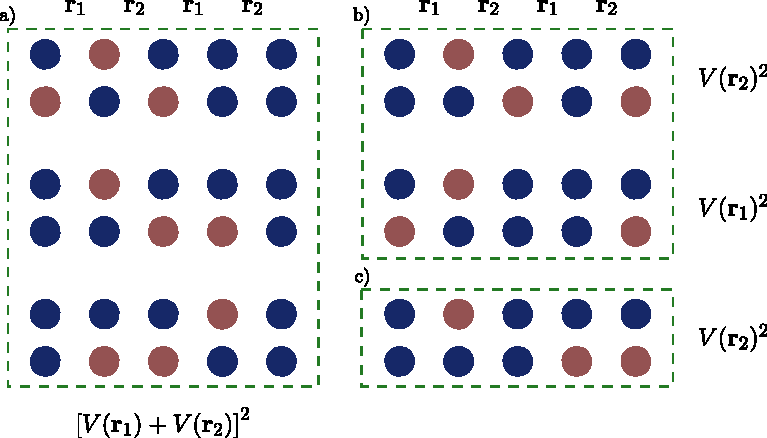
\includegraphics{pictures/SWT_calc.pdf}
    \caption{\textbf{Coupling schemes.} There are different ways double excited states couple to the single excited ones. The top row always depicts a state of the single, while the bottom row depicts a state of the double excited subspace. Generally configurations of two different subspaces are coupled to each other, when for two neighboring atoms one configuration has the inverted excitation scheme with respect to the other. I assign them to three categories. The first category is depicted in a). It couples two neighboring atoms twice. In the picture all possible cases are shown. For b) only two atoms couple two each other. Here the coupling takes place at a pair of $\ket{e}$ and $\ket{g}$ in both configurations. If the excitation in the single excitation subspace is at position $2<i<N-1$, there are $N-4$ different states in the double excited subspace that contribute a term $V(\mathbf{r}_1)^2$ and the same number for $V(\mathbf{r}_2)^2$. Category c) couples two unexcited sites in the single excitations subspace to two excited sites in the double excited subspace. For this case there are $N/2-2$ states that contribute $V(\mathbf{r}_1)^2$ and  $N/2-2$ states that contribute $V(\mathbf{r}_2)^2$, if the single excited state is is excited at atom $2<i<N-1$.}
    \label{fig:SWT_schemes}
\end{figure}
In the following the effective Hamiltonian will be calculated for the specific configuration we are looking at. We consider a one-dimensional staggered chain of $N$ atoms, where the atoms are separated by alternating distances $\mathbf{r}_1$ and $\mathbf{r}_2$. For a single atom there are only two states available, excited $\ket{e}$ and unexcited $\ket{g}$. The states $\ket{i}$, which are summed over, represent the states where only atom $i$ is excited and the others are in the unexcited state. Going to a regime where only nearest neighbor interactions contribute we can write using the coupling schemes of \figref{fig:SWT_schemes}
\begin{align*}
    H_{\text{eff},2}&= \sum_{i=1}^N\tilde{V}_i\,\ket{i}\bra{i}\\
    \tilde{V}_i &=-\frac{1}{\Delta}\,\begin{cases}
        3\,\left[V(\mathbf{r}_1)+V(\mathbf{r}_2)\right]^2+(N-4+\frac{N}{2}-2)\,V^2(\mathbf{r}_1)+(N-4+\frac{N}{2}-2)\,V^2(\mathbf{r}_2)&\text{if}\;1\neq i\neq N\\\\
        \left[V(\mathbf{r}_1)+V(\mathbf{r}_2)\right]^2+(N-3+\frac{N}{2}-1)\,V^2(\mathbf{r}_1)+(\frac{N}{2}-1)\,V^2(\mathbf{r}_2)&\text{if}\;i=1\\\\
        2\,\left[V(\mathbf{r}_1)+V(\mathbf{r}_2)\right]^2+(N-3+\frac{N}{2}-2)\,V^2(\mathbf{r}_1)+(N-4+\frac{N}{2}-1)\,V^2(\mathbf{r}_2)&\text{if}\;i=2\\\\
        2\,\left[V(\mathbf{r}_1)+V(\mathbf{r}_2)\right]^2+(N-4+\frac{N}{2}-1)\,V^2(\mathbf{r}_1)+(N-3+\frac{N}{2}-2)\,V^2(\mathbf{r}_2)&\text{if}\;i=N-1\\\\
        \left[V(\mathbf{r}_1)+V(\mathbf{r}_2)\right]^2+(\frac{N}{2}-1)\,V^2(\mathbf{r}_1)+(N-3+\frac{N}{2}-1)\,V^2(\mathbf{r}_2)&\text{if}\;i=N
    \end{cases}
\end{align*}
% There is actually another case distinction necessary for $i=2$ and $i=N-1$, this will be clearer later.
The part involving interactions within the same subspace can be written as 
\begin{align*}
    P_0VP_0&= \sum_{\substack{i=1\\j=i+1}}^{N-1} V(\mathbf{r}_{i,j})\,\sigma^+_i\sigma^-_j+\text{h.c.},
\end{align*}
where $\mathbf{r}_{i,j}$ is the distance between the $i$th and $j$th site. I now also want to write $H_{\text{eff},2}$ in terms of a sum of two atom operators. Therefore I introduce the projectors $n^e_i=\ket{e}_i\bra{e}_i$ and $n^g_i=\ket{g}_i\bra{g}_i$.
\begin{align*}
    H_{\text{eff},2}&=\sum_{\substack{i=1\\j=i+1}}^{N-1}V^2(\mathbf{r}_{i,j})\,(n^e_in^g_j + n^g_in^e_j + n^g_in^g_j)+\sum_{i=2}^{N-1}\left[ V(\mathbf{r}_{i-1,i})+V(\mathbf{r}_{i,i+1}) \right]^2 \, n^g_{i-1}n^e_in^g_{i+1}\\ &+\sum_{i=3}^{N-1} \left[ V(\mathbf{r}_{i-2,i-1})+V(\mathbf{r}_{i-1,i}) \right]^2 \, n^g_{i-2}n^g_{i-1}n^e_{i} 
    +\sum_{i=2}^{N-2} \left[ V(\mathbf{r}_{i,i+1})+V(\mathbf{r}_{i+1,i+2}) \right]^2 \, n^e_{i}n^g_{i+1}n^g_{i+2} \\
    &+ \left[ V(\mathbf{r}_{1,2})+V(\mathbf{r}_{2,3}) \right]^2 n^e_1n^g_2n^g_3 + \left[ V(\mathbf{r}_{N-2,N-1})+V(\mathbf{r}_{N-1,N}) \right]^2 n^g_{N-2}n^g_{N-1}n^e_{N}
\end{align*}
A last step is possible since in the single excitation subspace terms like $n^e_in^g_j$ simplify to just $n^e_i$.
\begin{align*}
    &= \sum_{i=2}^{N-1}\left(V^2(\mathbf{r}_{i-1,i})+V^2(\mathbf{r}_{i,i+1})+\left[ V(\mathbf{r}_{i-1,i})+V(\mathbf{r}_{i,i+1}) \right]^2 \right)\,n^e_i \\&+ \sum_{i=3}^{N-1} \left[ V(\mathbf{r}_{i-2,i-1})+V(\mathbf{r}_{i-1,i}) \right]^2\, n^e_i +\sum_{i=2}^{N-2} \left[ V(\mathbf{r}_{i,i+1})+V(\mathbf{r}_{i+1,i+2}) \right]^2\,n^e_i\\
    &+ \left( V^2(\mathbf{r}_{1,2}) + \left[ V(\mathbf{r}_{1,2})+V(\mathbf{r}_{2,3}) \right]^2 \right)\,n^e_1 + \left( V^2(\mathbf{r}_{N-1,N})+ \left[ V(\mathbf{r}_{N-2,N-1})+V(\mathbf{r}_{N-1,N}) \right]^2\right)\,n^e_N\\
    &+ \sum_{i=1}^{N-1} V(\mathbf{r}_{i,i+1})\,n^g_in^g_{i+1}
\end{align*}
\subsection*{First order approximation}
For the first approach I will continue with the Hamiltonian up to first order in the dipole interaction, i.e. without $H_{\text{eff},2}$. The phonons are introduced by again expanding the interaction up to second order. I will restrict the consideration also to the constant phonon excitation subspace. For this reason the first order expansion of the dipole interaction will be ignored, as it couples subspaces with different phonon numbers. The Hamiltonian thus reads
\begin{align*}
    H&= \sum_{i=1}^{N-1}\left[V(\mathbf{r}_{i,i+1})+\sum_{n,m\in\{i,i+1\}}\frac{\partial^2V(\mathbf{r}_{i,i+1})}{\partial\mathbf{r}_{n}\partial\mathbf{r}_m}\,\delta\mathbf{\hat{r}}_n\delta\mathbf{\hat{r}}_m\right]\,\sigma_i^+\sigma_{i+1}^-+\text{h.c.}
\end{align*}
The hats in $\delta\mathbf{\hat{r}}$ indicates operators. Here also the operators are projected on the constant phonon subspace. What has to be accounted for is that this second order expansion is only valid if the displacement is small, which means $1/\sqrt{m\omega}\ll1$ as $||a||\sim1$.
\begin{align*}
    \left| 1- \frac{V(\mathbf{r}+\delta\mathbf{r})}{V(\mathbf{r})} \right|&\ll 1\\
    \left| \frac{\partial^2 V(\mathbf{r})}{\partial\mathbf{r}^2}\,\delta\mathbf{r}^2 \right|&\ll\left|V(\mathbf{r})\right|
\end{align*}
When quantizing the displacements to phonon operators $\delta\mathbf{r}^2\rightarrow \frac{2}{m\omega}\,a^\dagger a$, one finds the condition 
\begin{align*}
    \frac{2}{m\omega}\, \left| \frac{\partial^2 V(\mathbf{r})}{\partial\mathbf{r}^2} \right|&\ll\left|V(\mathbf{r})\right|,
\end{align*}
as $a^\dagger a$ is of the order of 1. 
\begin{figure}[H]
    \centering
    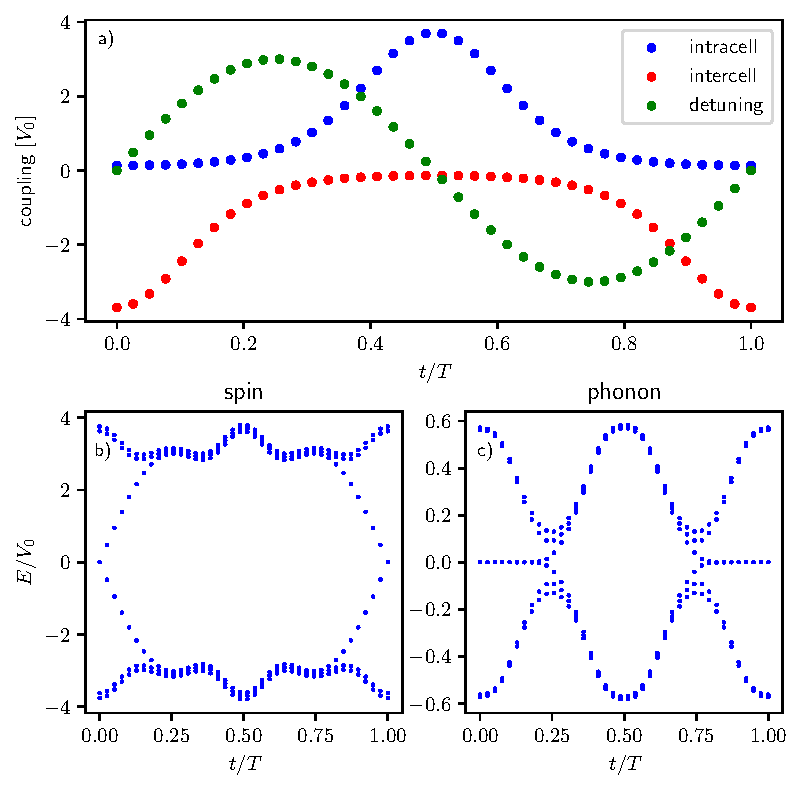
\includegraphics{pictures/rice_mele_protocol.pdf}
    \caption{\textbf{Spin transfer protocol.} In a the course of the interaction during the transfer protocol is shown. b-c show the spectrum of the spin and phonon Hamiltonian respectively during the pump cycle each for one excitation in the respective degrees of freedom. For the spin Hamiltonian a pure dipole dipole interaction is used, where the dipole moments of the atoms are orientated in way that puts the interactions within the same sublattice to zero. This choice improves the accuracy of the nearest neighbor assumption. The phonon spectrum is received by the methods used in the previous chapters. It therefore depicts a scenario without spin degrees of freedom.}
    \label{fig:pump_protocol}
\end{figure}
As a next step I want to first discard the phonon dynamics and realize a transfer protocol for a spin excitation through the chain. For this purpose I implement a Rice-Mele model configuration for the chain of Rydberg atoms. This is achieved by including an onsite potential with alternating sign of the form
\begin{align*}
    H_\text{OS}= \sum_{i=1}^N(-1)^i \,\Delta\,\sigma^+_i\sigma^-_i.
\end{align*}
Note that the detuning $\Delta$ is now a different parameter from above. By changing the position and detuning in an adiabatic cyclic way, one can implement a transfer protocol, which is depicted in \figref{fig:pump_protocol}. The system is initialized with the eigenstate of the spin Hamiltonian located at the edge. This is possible, as I start the transfer protocol in the topological phase. After the the transfer period I compare the evolved state with the target state, which is the eigenstate located at the other side. I use a chain of six atoms in total. The resulting fidelity between final and target state for this protocol is $0.9996$.\\\\
I can now compare which influence the introduction of photons has on the transfer quality. Therefore I test the effect of four different phonon initial states on the transfer process. The different initial phonon states can be read of \figref{fig:transfer_trajectories}. \figref{fig:fidelity} shows that the evolvement of the phonon degrees of freedom does not change the quality of the transfer to a very considerable portion, where I investigated how the strength of the phonon-phonon interactions effect
the fidelity of final and target state. In \figref{fig:2phonon_exc_traj} I show the time evolution of the phononic degrees of freedom for two initial phonon excitations.


\begin{figure}[H]
    \centering
    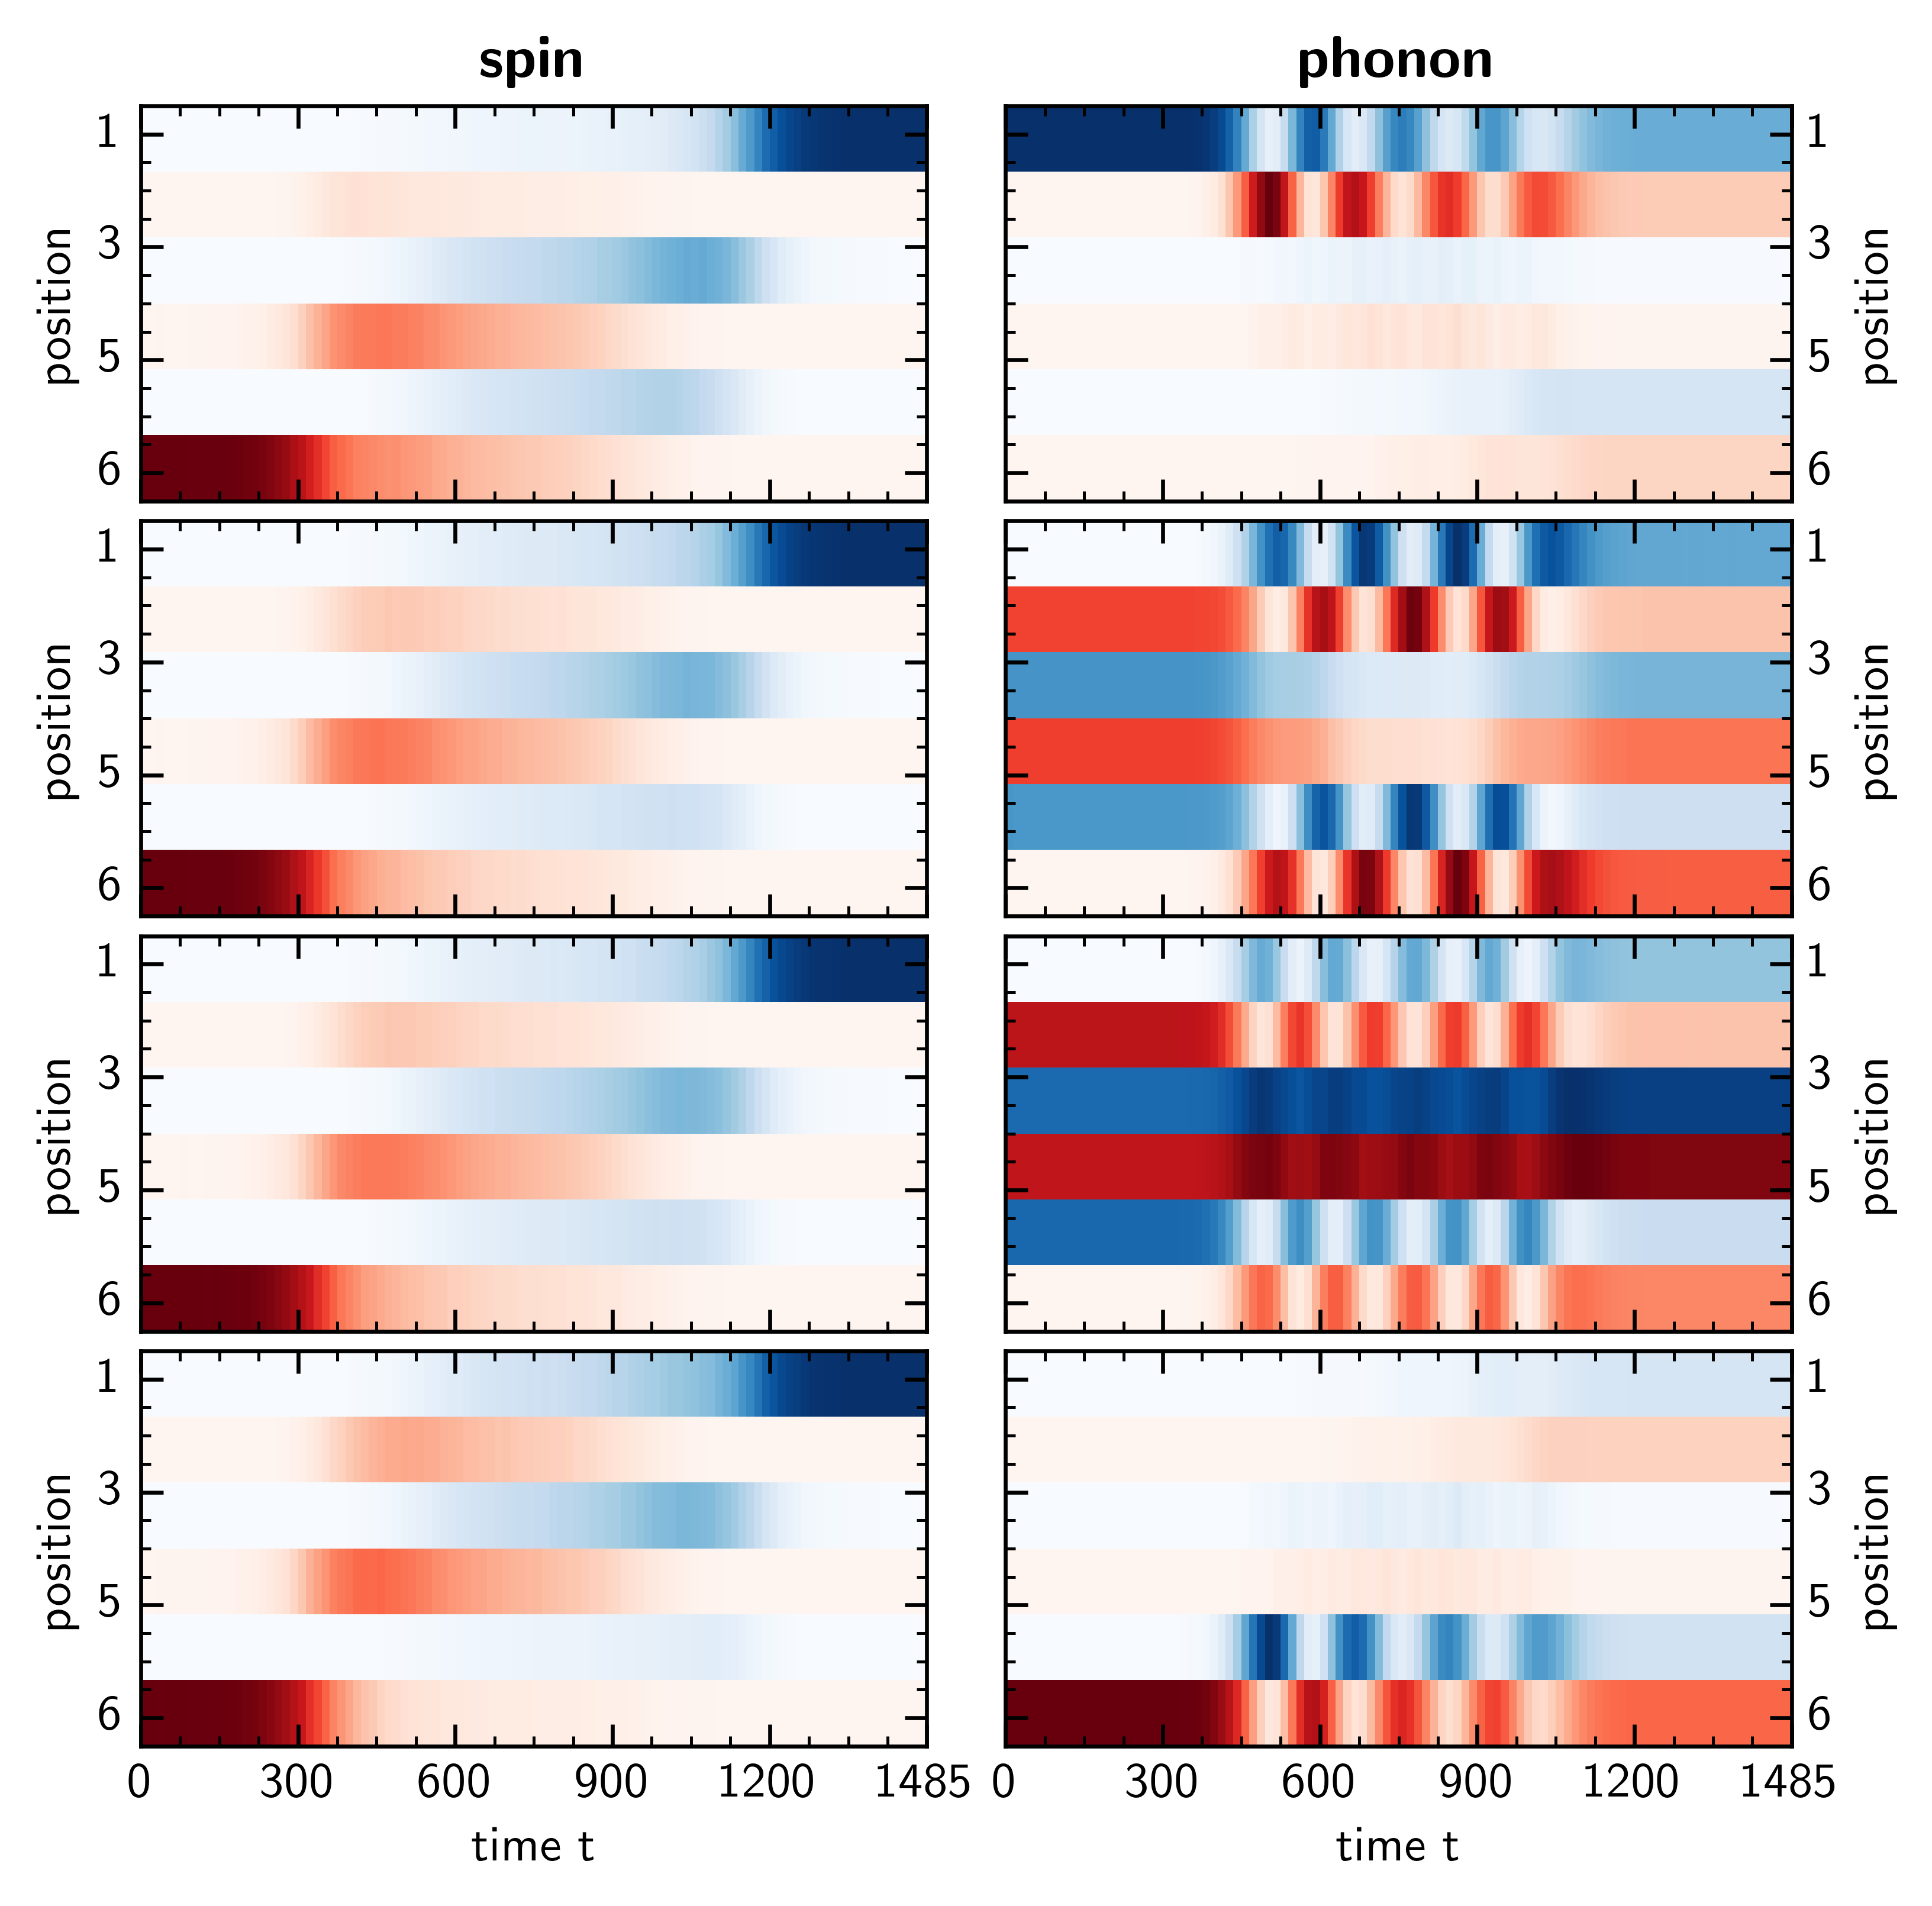
\includegraphics{pictures/spin_phonon_traj_colormap_phintc_rescale100.png}
    \caption{\textbf{Spin transfer process.} The time evolution of the spin and phonon degrees of freedom is depicted during the adiabatic transfer protocol. For the same transfer protocol the system was prepared in different initial phonon configurations, which stored one excitation in total.}
    \label{fig:transfer_trajectories}
\end{figure}

\begin{figure}[H]
    \centering
    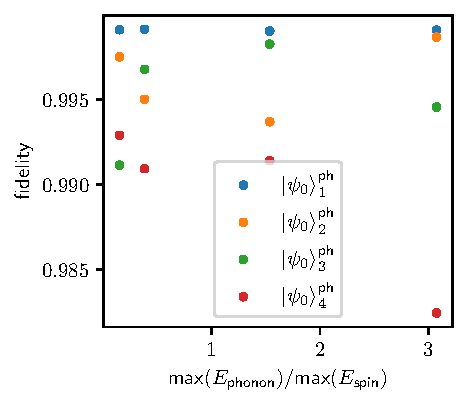
\includegraphics{pictures/fidelity_coupling_strengths.pdf}
    \caption{\textbf{Fidelity in dependence of phonon interaction strength.} For the 4 initial phonon configurations introduced in \figref{fig:transfer_trajectories} (the labeling runs from top to bottom) different rations of spin dipole interactions to phonon interactions are chosen. The fidelity between the final and target state is shown in dependence of interaction ratio and initial phonon state.}
    \label{fig:fidelity}
\end{figure}

\begin{figure}[H]
    \centering
    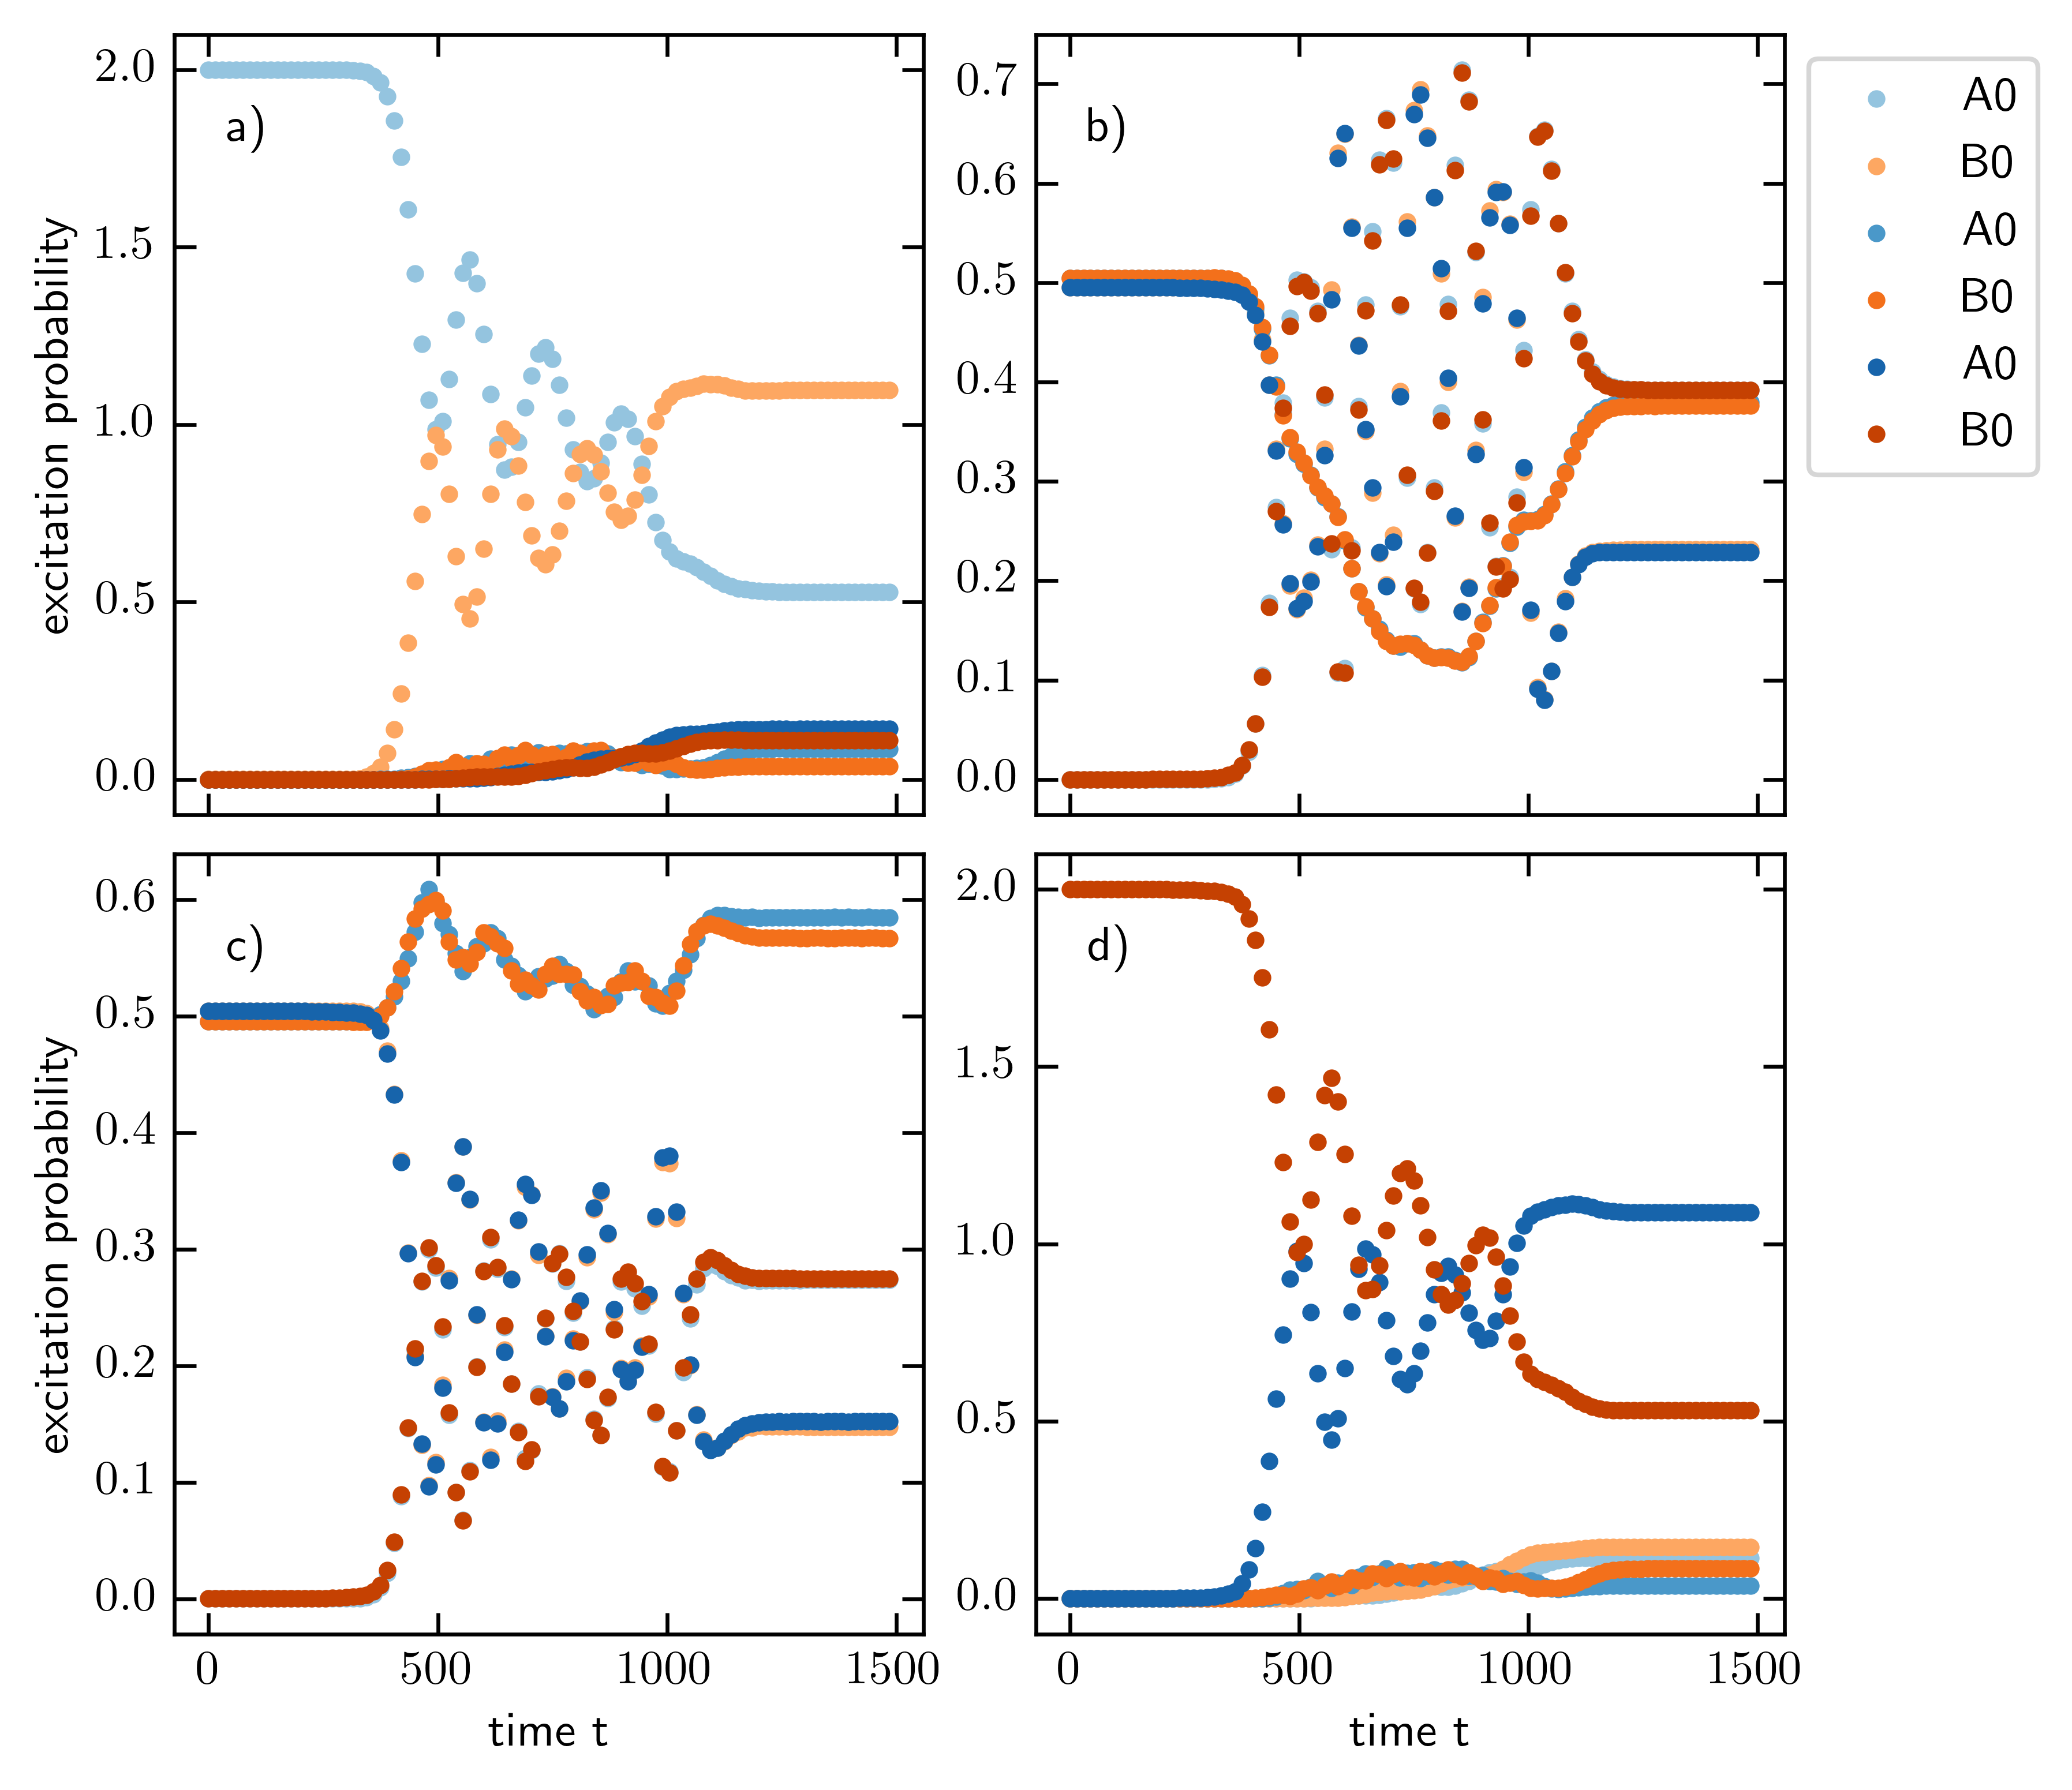
\includegraphics{pictures/spin_phonon_traj_lines_phintc_rescale100_2ph.png}
    \caption{\textbf{Phonon evolution for two excitations.} For two phonon excitations the evolution of the phonons during the transfer period is depicted.}
    \label{fig:2phonon_exc_traj}
\end{figure}


\section*{Winding number of the spin-phonon coupled Hamiltonian}
Next I want to determine the topological phase of the Hamiltonian where spin and and motional degrees of freedom are coupled in first order Schrieffer-Wolff approximation. I will again consider only nearest neighbor interaction and will also constrain the dynamics to the single excitation subspace, both in spin and phonon degrees of freedom. For this purpose I will write the interactions in terms of fermionic spin and phonon operators. $a_i$ and $b_i$ ($p_{A,i}$ and $p_{B,i}$) are spin (phonon) annihilation operators acting, respectively, on the sublattice $A$ and $B$ sites in unit cell $i$. The Hamiltonian then reads 
\begin{align*}
    H &= H_\text{sp}+H_\text{spph}\\
    \text{with}\quad H_\text{sp} &= \sum_i V_1\,a_i^\dagger b_i + V_2\,b_i^\dagger a_{i+1} +\text{h.c.}\\
    H_\text{spph}&= \sum_i V_3\,\left[ p_{A,i}^\dagger p_{B,i} + p_{B,i}^\dagger p_{A,i} - p_{A,i}^\dagger p_{A,i} - p_{B,i}^\dagger p_{B,i} \right]\,a_i^\dagger b_i +\text{h.c.}\\
    &+\sum_i V_4\,\left[ p_{A,i+1}^\dagger p_{B,i} + p_{B,i}^\dagger p_{A,i+1} - p_{A,i+1}^\dagger p_{A,i+1} - p_{B,i}^\dagger p_{B,i} \right]\,a_{i+1}^\dagger b_i +\text{h.c.}
\end{align*}
Here the intracell couplings $V_1$, $V_3$, and the intercell couplings $V_2$, $V_4$ are constants which depend on the parameters distance and dipole moment. Transforming this Hamiltonian into momentum space by simply performing a Fourier transform of every operator does not simplify the description and does not allow for an analysis of the winding number.

But by building collective operators of spin and phonon degrees of freedom one is able to make use of the one dimensional character of the chain and achieve a momentum space Hamiltonian with decoupled momenta. First I restrict myself to the spin phonon coupled term of the Hamiltonian. I group all operators in $H_\text{spph}$ acting on the same sublattice together and combine them into one operator, defined on an adapted space. By this procedure I get a couple of new operators. All of them act on the same space, which is defined on one site.
\begin{align*}
    \begin{pmatrix}
        s_i^\uparrow p_i^\uparrow\\
        s_i^\uparrow p_i^\downarrow\\
        s_i^\downarrow p_i^\uparrow\\
        s_i^\downarrow p_i^\downarrow
    \end{pmatrix}=\vcentcolon \begin{pmatrix}
        \ket{1}\\
        \ket{2}\\
        \ket{3}\\
        \ket{4}
    \end{pmatrix}
\end{align*}

For $D\in\{A,B\}$ and $d\in\{a,b\}$ I define
\begin{align*}
    c^{\bar{D},D}_i\vcentcolon&=p_{D,i}^\dagger d_i = \ket{3}\bra{2}\\
    c^{D,\bar{D}}_i\vcentcolon&=p_{D,i}\,d_i^\dagger = \ket{2}\bra{3}\\
    c^{\bar{D},\bar{D}}_i\vcentcolon&=p_{D,i}^\dagger d_i^\dagger = \ket{1}\bra{4}\\
    c^{D,D}_i\vcentcolon&=p_{D,i}\, d_i = \ket{4}\bra{1}\\
    c^{\bar{D}}_i\vcentcolon&= d_i^\dagger = \ket{1}\bra{3}+\ket{2}\bra{4}\\
    c^{D}_i\vcentcolon&= d_i = \ket{3}\bra{1}+\ket{4}\bra{2}\\
    c^{\bar{D},D,D}_i\vcentcolon&=p_{D,i}^\dagger p_{D,i}\, d_i = \ket{3}\bra{1}\\
    c^{\bar{D},D,\bar{D}}_i\vcentcolon&=p_{D,i}^\dagger p_{D,i}\, d_i^\dagger = \ket{1}\bra{3}\,
\end{align*}
what lets the Hamiltonian read
\begin{align*}
    H_\text{spph}&= \sum_i V_3\,\left[ c_i^{\bar{A},\bar{A}}\,c_i^{B,B} + c_i^{A,\bar{A}}\,c_i^{\bar{B},B} - c_i^{\bar{A},A,\bar{A}}\,c_i^{B} - c_i^{\bar{A}}\,c_i^{\bar{B},B,B}\right] +\text{h.c.}\\
    &+ \sum_i V_4\,\left[ c_{i+1}^{\bar{A},\bar{A}}\,c_i^{B,B} + c_{i+1}^{A,\bar{A}}\,c_i^{\bar{B},B} - c_{i+1}^{\bar{A},A,\bar{A}}\,c_i^{B} - c_{i+1}^{\bar{A}}\,c_i^{\bar{B},B,B}\right] +\text{h.c.}
\end{align*}
Because of the single excitation restriction, exactly one phonon and spin has to be present at the two neighboring sites for a term acting on those two neighboring sites to contribute. Therefore the combined space of the two neighboring sites collapses to the dimensin of the one site space, represented by the basis
\begin{align*}
    \begin{pmatrix}
        s_1^\uparrow p_1^\uparrow \; s_2^\downarrow p_2^\downarrow\\
        s_1^\uparrow p_1^\downarrow\; s_2^\downarrow p_2^\uparrow\\
        s_1^\downarrow p_1^\uparrow\; s_2^\uparrow p_2^\downarrow\\
        s_1^\downarrow p_1^\downarrow\; s_2^\uparrow p_2^\uparrow
    \end{pmatrix}
\end{align*}
The Hamiltonian in $k$-space then reads
\begin{align*}
    H_\text{spph}&= \sum_k V_3\,\left[ c_k^{\bar{A},\bar{A}}\,c_k^{B,B} + c_k^{A,\bar{A}}\,c_k^{\bar{B},B} - c_k^{\bar{A},A,\bar{A}}\,c_k^{B} - c_k^{\bar{A}}\,c_k^{\bar{B},B,B}\right] +\text{h.c.}\\
    &+ \sum_k V_4\,e^{ika}\,\left[ c_k^{\bar{A},\bar{A}}\,c_k^{B,B} + c_k^{A,\bar{A}}\,c_k^{\bar{B},B} - c_k^{\bar{A},A,\bar{A}}\,c_k^{B} - c_k^{\bar{A}}\,c_k^{\bar{B},B,B}\right] +\text{h.c.}\\
    &= \sum_k \left(V_3+V_4\,e^{ika}\right)\,\left[ c_k^{\bar{A},\bar{A}}\,c_k^{B,B} + c_k^{A,\bar{A}}\,c_k^{\bar{B},B} - c_k^{\bar{A},A,\bar{A}}\,c_k^{B} - c_k^{\bar{A}}\,c_k^{\bar{B},B,B}\right] +\text{h.c.}\\
    &=\vcentcolon \sum_k H_\text{spph}^k
\end{align*}
The blocks in $k$-space then read
\begin{align*}
    H_\text{spph}= \begin{pmatrix}
        0 & 0 & -(V_3+V_4\,e^{ika}) & V_3+V_4\,e^{ika}\\
        0 & 0 & V_3+V_4\,e^{ika} & -(V_3+V_4\,e^{ika})\\
        -(V_3+V_4\,e^{-ika}) & V_3+V_4\,e^{-ika} & 0 & 0 \\
       V_3+V_4\,e^{-ika} & -(V_3+V_4\,e^{-ika}) & 0 & 0         
    \end{pmatrix}
\end{align*}
When considering the total Hamiltonian including $H_\text{sp}$ one has to expand the space for the collective operators as now the Hamiltonian does not only couple states where spin and phonon excitations are next to each other. But only two new states have to be introduced, $s_1^\uparrow p_1^\downarrow \; s_2^\downarrow p_2^\downarrow$ and $s_1^\downarrow p_1^\downarrow\; s_2^\uparrow p_2^\downarrow$. The basis is now family
\begin{align*}
    \begin{pmatrix}
        s_1^\uparrow p_1^\uparrow \; s_2^\downarrow p_2^\downarrow\\
        s_1^\uparrow p_1^\downarrow\; s_2^\downarrow p_2^\uparrow\\
        s_1^\uparrow p_1^\downarrow \; s_2^\downarrow p_2^\downarrow\\
        s_1^\downarrow p_1^\uparrow\; s_2^\uparrow p_2^\downarrow\\
        s_1^\downarrow p_1^\downarrow\; s_2^\uparrow p_2^\uparrow\\
        s_1^\downarrow p_1^\downarrow\; s_2^\uparrow p_2^\downarrow
    \end{pmatrix}=\vcentcolon \begin{pmatrix}
        \ket{1}\\
        \ket{2}\\
        \ket{3}\\
        \ket{4}\\
        \ket{5}\\
        \ket{6}
    \end{pmatrix}
\end{align*}
In this basis the spin Hamiltonian in momentum space $H_\text{sp}^k$ reads
\begin{align*}
    H_\text{sp}^k &= \begin{pmatrix}
        0&\alpha\\
        \alpha^\dagger&0
    \end{pmatrix}\\
    \text{with}\quad\alpha&= \left(V_1+V_2\,e^{ika}\right)\,\begin{pmatrix}
        1&0&0\\
        0&1&0\\
        0&0&1
    \end{pmatrix}
\end{align*}
The total Hamiltonian in momentum space thus reads
\begin{align*}
    H^k &= \begin{pmatrix}
        0&\beta\\
        \beta^\dagger&0
    \end{pmatrix}\\
    \text{with}\quad\beta&=\begin{pmatrix}
        V_1-V_3+(V_2-V_4)\,e^{ika}&V_3+V_4\,e^{ika}&0\\
        V_3+V_4\,e^{ika}&V_1-V_3+(V_2-V_4)\,e^{ika}&0\\
        0&0&V_1+V_2\,e^{ika}
    \end{pmatrix}
\end{align*}
The eigenvalues of $\beta$ are
\begin{align*}
    \beta_1 &= V_1-2\,V_3+(V_2-2\,V_4)\,e^{ika}\\
    \beta_2 = \beta_3 &= V_1+V_2\,e^{ika}
\end{align*}
\subsection*{Problems}
The main practical problem is that the total Hamiltonian is heavily degenerate $\sim N$. The winding number can however only take values between $0$ and $3$. Which eigenvalues are the topological protected ones?

This might be not due to an erroneous derivation of the momentum space Hamiltonian. But I don't know. At first glance there is a problem with the kernel of the Hamiltonian. In real space it has a finite dimension of the magnitude of $N$. But in momentum space the kernel seems to vanish. I think the reason is that I only considered a basis for the combined coupling operators, which actually couple, hence discarding the kernel. But I think this is no unusual proceed. I don't know if the winding number is valid for degenerate Hamiltonians. 

\begin{itemize}
\item Go to higher dimensions, e.g. transport on the closed surface of a 2D-lattice
\item Spin-phonon coupling:%\\
% $H = H_\text{sp}+ H_\text{sp-ph}$
\begin{itemize}
\item What effect has the spin-phonon coupling on transport performance?
\item Is it possible to transport both spins and phonons simultaneously?
\end{itemize}
\end{itemize}
\newpage
\subsection*{Spin-phonon coupling} 
$$H=\sum_j H_\text{ph}^{j,j+1} a_j^\dagger a_{j+1} + \text{h.c.}$$
with 
$$H_\text{ph}^{j,j+1}=V_{j,j+1}^\text{der}\left(p_j^\dagger p_{j+1}+p_{j+1}^\dagger p_{j}-p_{j}^\dagger p_{j}-p_{j+1}^\dagger p_{j+1}\right)$$
$a_j$ and $p_j$ are spin and phonon annihilation operators respectively.
\subsubsection*{Attempt of analytic solution for the time evolution (3 atoms)}
I'm considering 3 atoms with the Hamiltonian 
\begin{align*}
H&=H_{12}a^\dagger b+H_{23}b^\dagger c +\text{h.c.}\\
\text{with}\quad H_{ij}&=p_i^\dagger p_{j}+p_{j}^\dagger p_{i}-p_{i}^\dagger p_{i}-p_{j}^\dagger p_{j}
\end{align*}
I want to calculate the time evolution of the occupation operator $a^\dagger a$.
$$a^\dagger a(t) = e^{iHt}a^\dagger a e^{-iHt}=\sum_n\frac{(it)^n}{n!} [H,a^\dagger a]_n=:\sum_n\frac{(it)^n}{n!}\,C_n$$
with $[H,a^\dagger a]_n = [H,[H,a^\dagger a]_{n-1}]$.
$$C_2 = 2 H_{12}^2 (a^\dagger a - b^\dagger b) + H_{23} H_{12} c^\dagger a + H_{12} H_{23} a^\dagger c $$ $$C_3 = (4 H_{12}^3 + H_{23}^2 H_{12}) b^\dagger a - (4 H_{12}^3 + H_{12} H_{23}^2) a^\dagger b - 3 H_{23} H_{12}^2 c^\dagger b + 3 H_{12}^2 H_{23} b^\dagger c $$

$$ C_4 = (8 H_{12}^4 + 2 H_{12} H_{23}^2 H_{12}) a^\dagger a - \left(8 H_{12}^4 + 4 H_{12}^2 H_{23}^2 + 4 H_{23}^2 H_{12}^2 \right) b^\dagger b + 6 H_{23} H_{12}^2 H_{23} c^\dagger c  $$$$+ (7 H_{23} H_{12}^3 + H_{23}^3 H_{12}) c^\dagger a + (7 H_{12}^3 H_{23} + H_{12} H_{23}^3) a^\dagger c$$
Concentrating on the odd indices one can determine a recursion relation for the coefficients of $a^\dagger b$ and $b^\dagger c$. 
\begin{align*}
    c_{ab}'&=H_{12}^2\,c_{ab}+c_{ab}\,(H_{12}^2+H_{23}^2)+2H_{12}\,c_{ab}^\dagger \,H_{12}-2H_{12}\,c_{bc}\,H_{23}-H_{12}H_{23}\,c_{bc}^\dagger  \\\\
    c_{bc}'&=(H_{12}^2+H_{23}^2)\,c_{bc}+c_{bc}\,H_{23}^2+2H_{23}\,c_{bc}^\dagger \,H_{23}-2H_{12}\,c_{ab}\,H_{23}-c_{ab}^\dagger\, H_{12}H_{23} 
\end{align*}
By redefining the coefficients as
$$c_{ab}=\vcentcolon H_{12}\,\alpha  ,\quad c_{bc}=\vcentcolon \beta\,H_{23}$$
one can reach at a slightly simpler recursion relation
$$\alpha_{n+1}=H_{12}^2\,\alpha_n +\alpha_n \,(H_{12}^2+H_{23}^2)+2\alpha_n ^\dagger \,H_{12}^2+2\beta_n\,H_{23}^2+H_{23}^2\,\beta_n^\dagger$$
$$\beta_{n+1} = (H_{12}^2+H_{23}^2)\,\beta_n + \beta_n\, H_{23}^2 + 2H_{23}^2\,\beta_n^\dagger + 2H_{12}^2\,\alpha_n + \alpha_n^\dagger\, H_{12}^2$$

\begin{figure}[H]
    \hspace*{-2.5cm}
    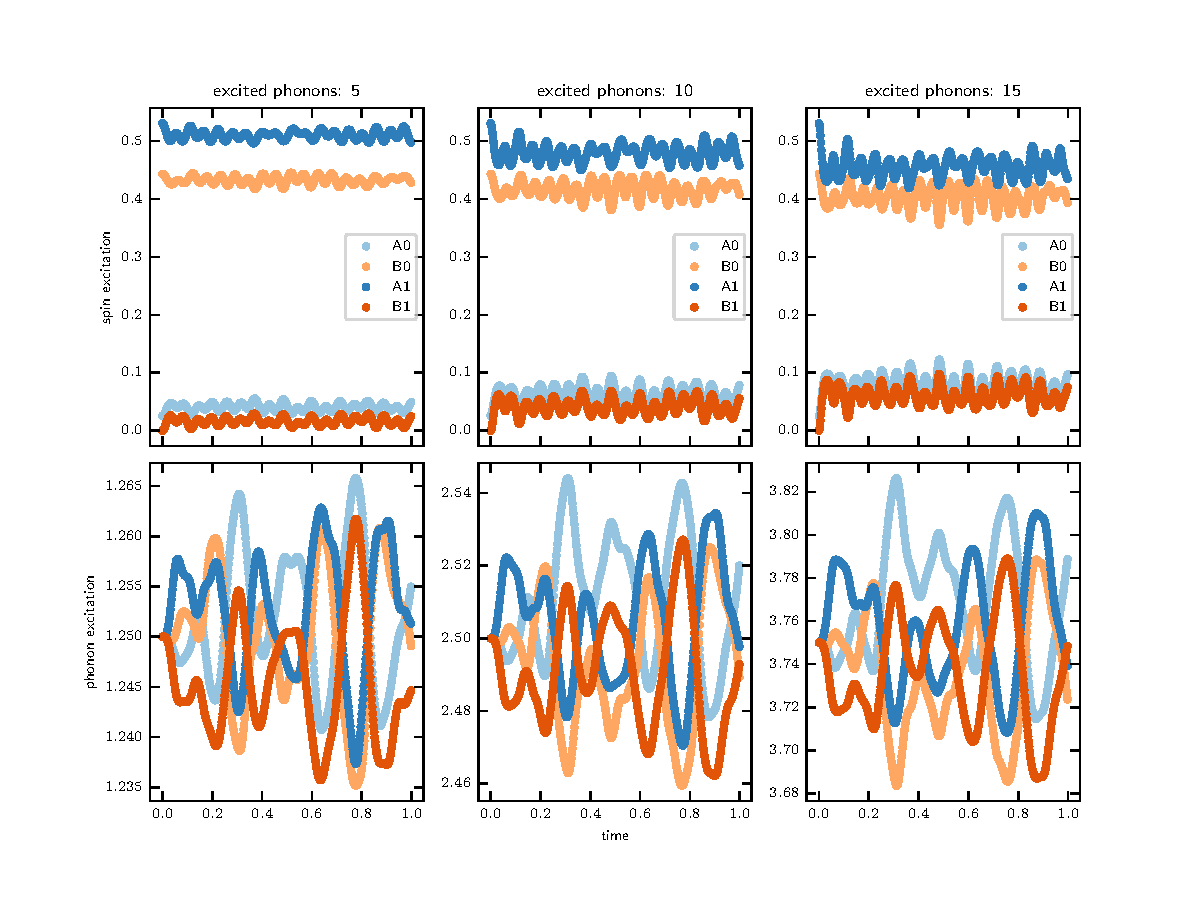
\includegraphics{pictures/chain4_only_coupling.pdf}
    \caption{\textbf{Evolution with only spin-phonon coupling term.}}
    % \label{fig:fidelity}
\end{figure}
\begin{figure}[H]
    \hspace*{-2.5cm}
    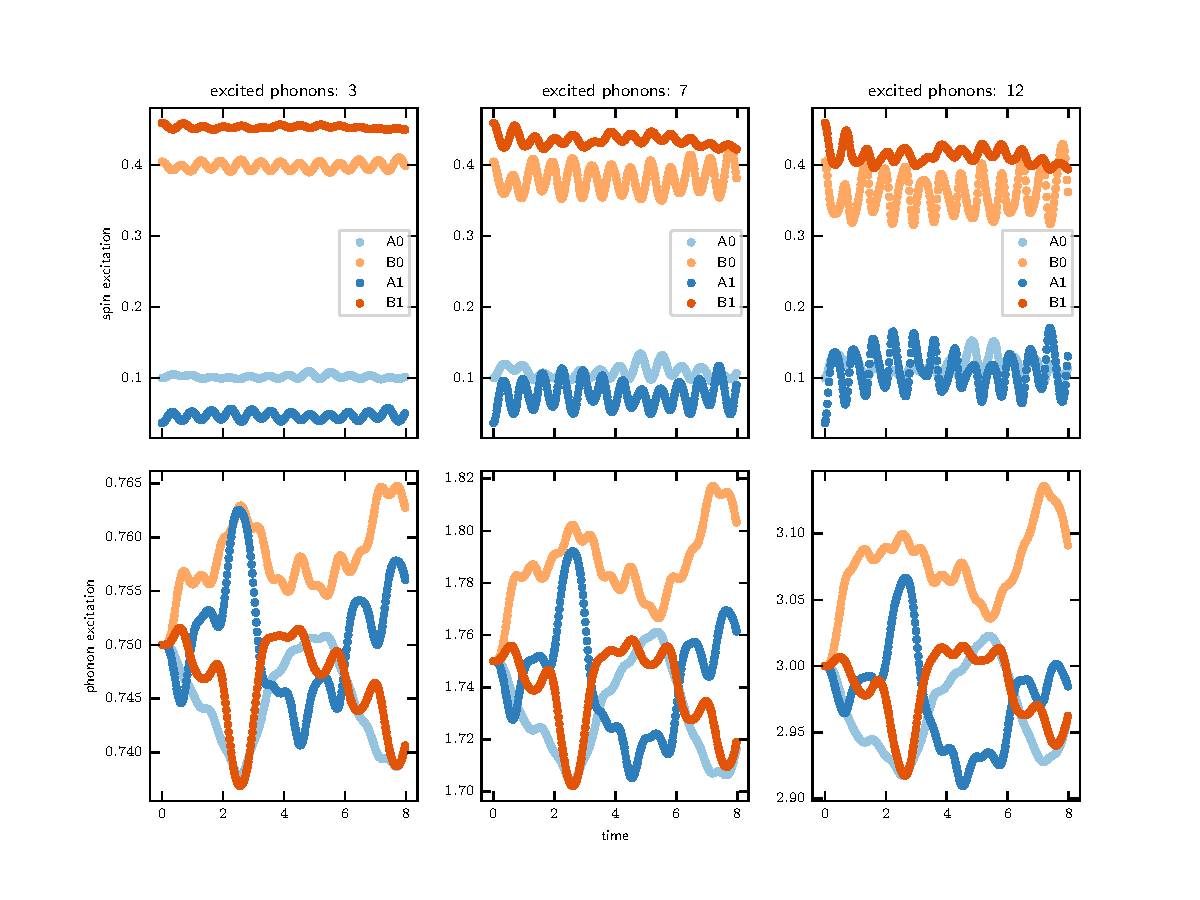
\includegraphics{pictures/chain4_spin_phonon_only.pdf}
    \caption{\textbf{Evolution with only spin-phonon coupling term.}}
    % \label{fig:fidelity}
\end{figure}
\begin{figure}[H]
    \hspace*{-2.5cm}
    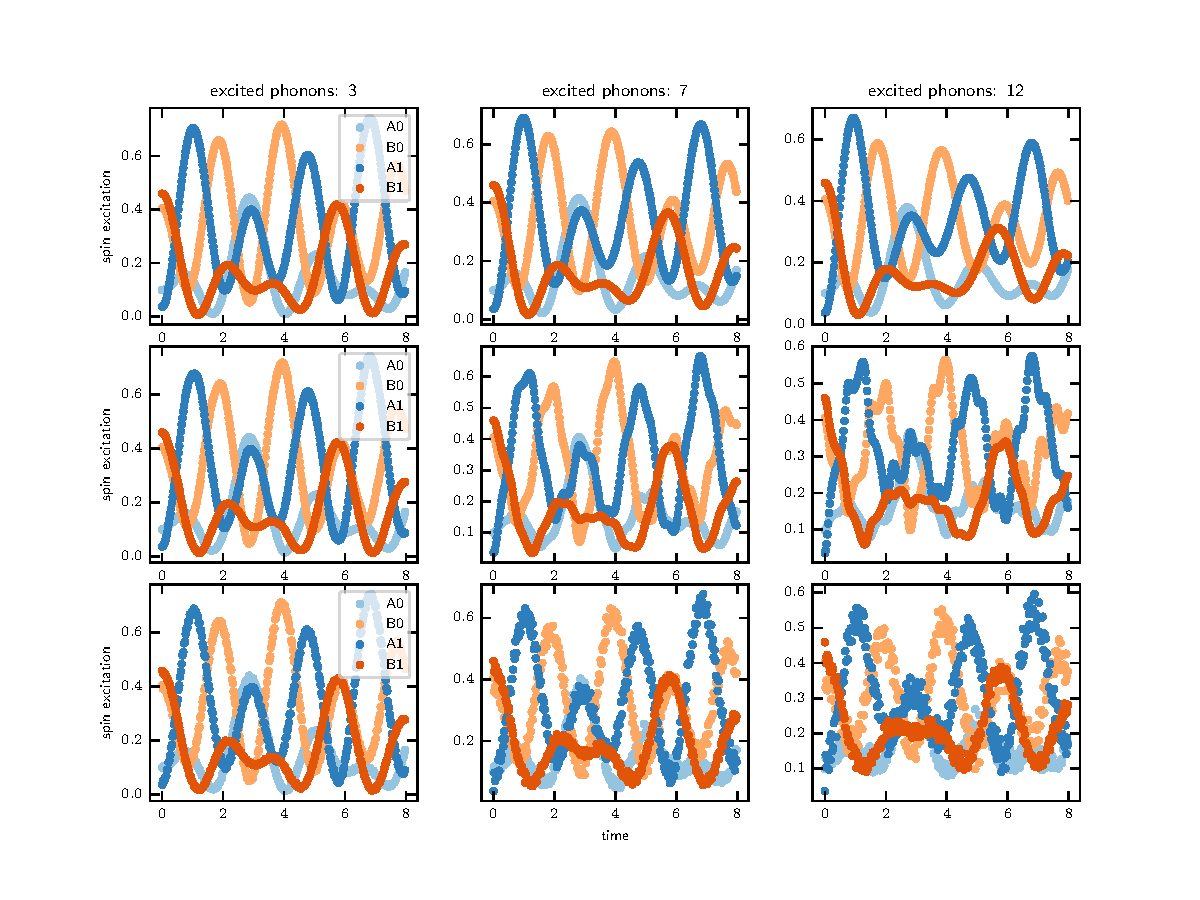
\includegraphics{pictures/chain4_free_evol_all_coupling.pdf}
    \caption{\textbf{Summary spin evolution}}
    % \label{fig:fidelity}
\end{figure}
\begin{figure}[H]
    \hspace*{-2.5cm}
    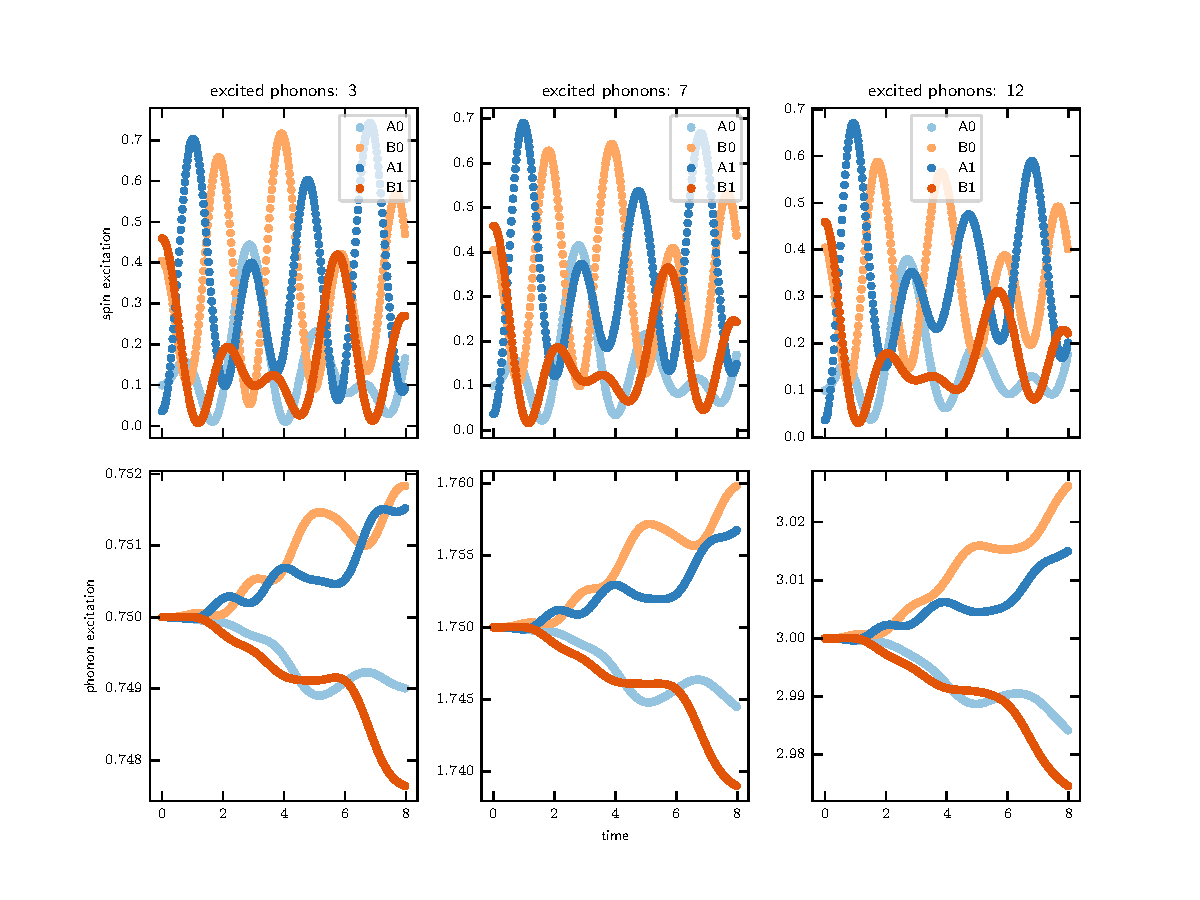
\includegraphics{pictures/chain4_free_evol_1spto1tenthcoupling.pdf}
    \caption{\textbf{Evolution with full Hamiltonian ratio spin only: coupling 10:1.}}
    % \label{fig:fidelity}
\end{figure}
\begin{figure}[H]
    \hspace*{-2.5cm}
    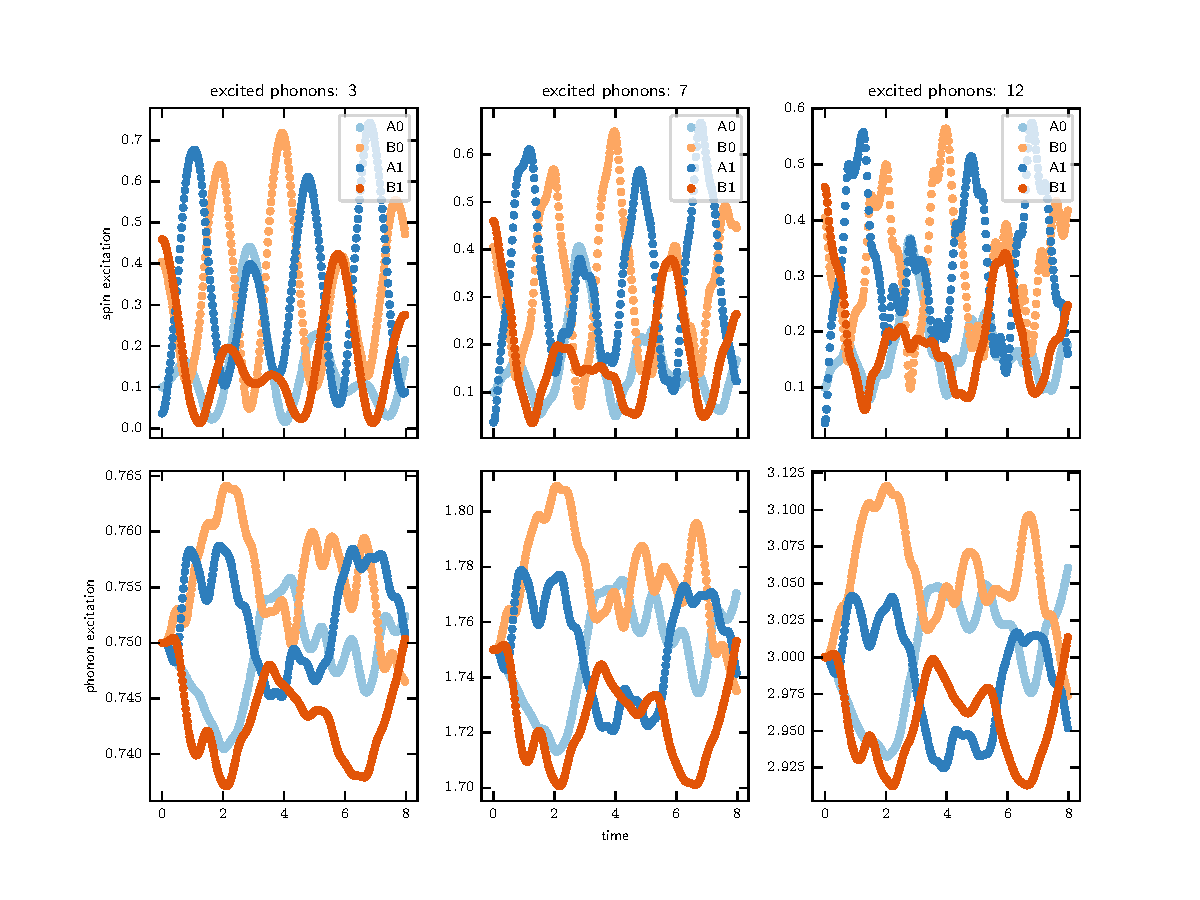
\includegraphics{pictures/chain4_free_evol_1spto1coupling.pdf}
    \caption{\textbf{Evolution with full Hamiltonian ratio spin only: coupling 1:1.}}
    % \label{fig:fidelity}
\end{figure}
\begin{figure}[H]
    \hspace*{-2.5cm}
    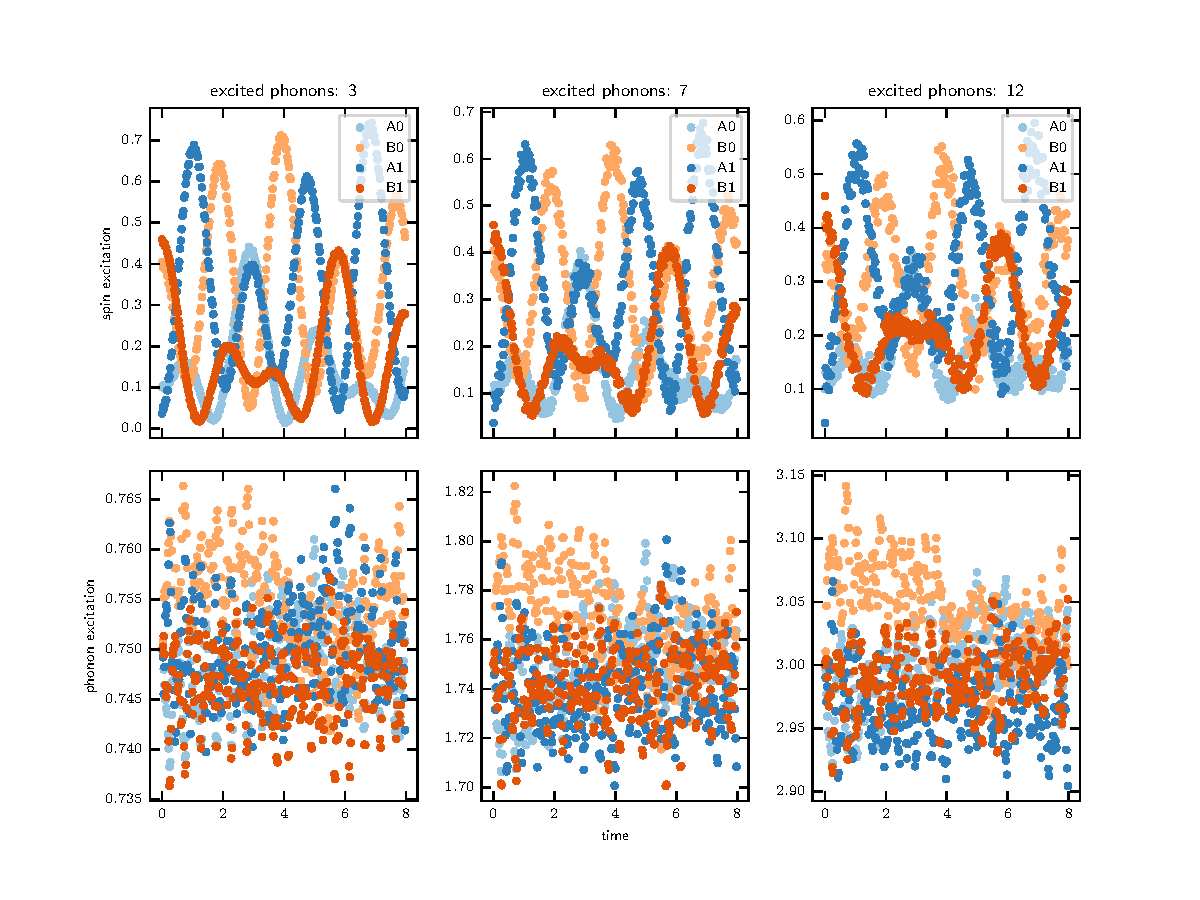
\includegraphics{pictures/chain4_free_evol_1spto10coupling.pdf}
    \caption{\textbf{Evolution with full Hamiltonian ratio spin only: coupling 1:10.}}
    % \label{fig:fidelity}
\end{figure}



\begin{figure}[H]
    \hspace*{-2.5cm}
    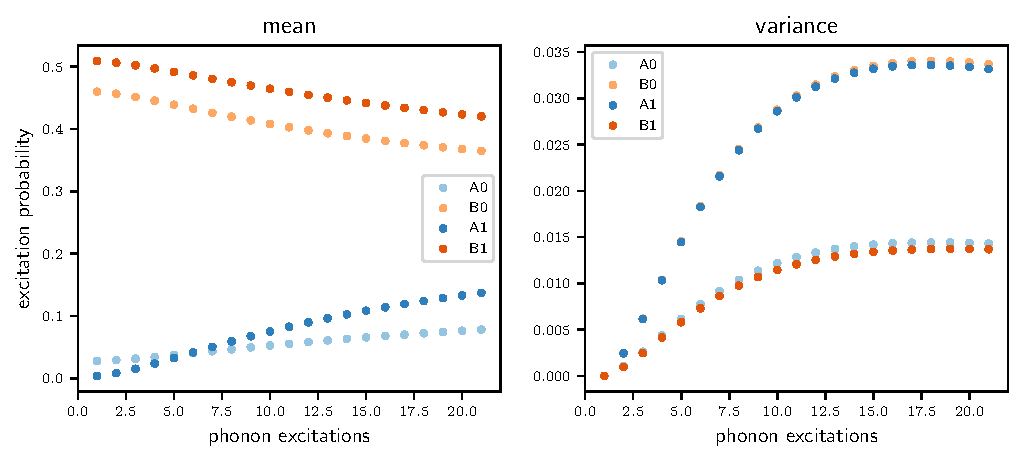
\includegraphics{pictures/chain4_spin_phonon_only_mean_variance.pdf}
    \caption{\textbf{spin-phonon coupling only.}}
    % \label{fig:fidelity}
\end{figure}
\begin{figure}[H]
    \hspace*{-2.5cm}
    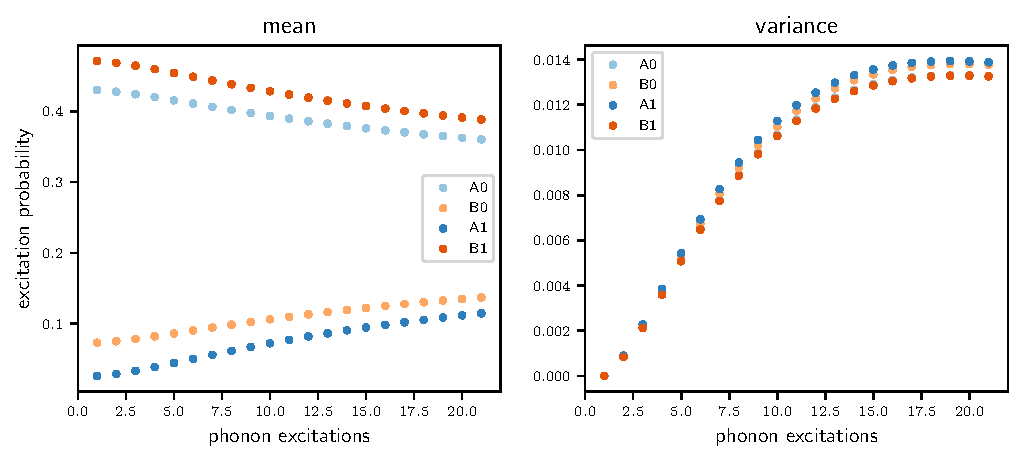
\includegraphics{pictures/chain4_spin_phonon_only_mean_variance2.pdf}
    % \caption{\textbf{spin-phonon coupling only.}}
    % \label{fig:fidelity}
\end{figure}
\begin{figure}[H]
    \hspace*{-2.5cm}
    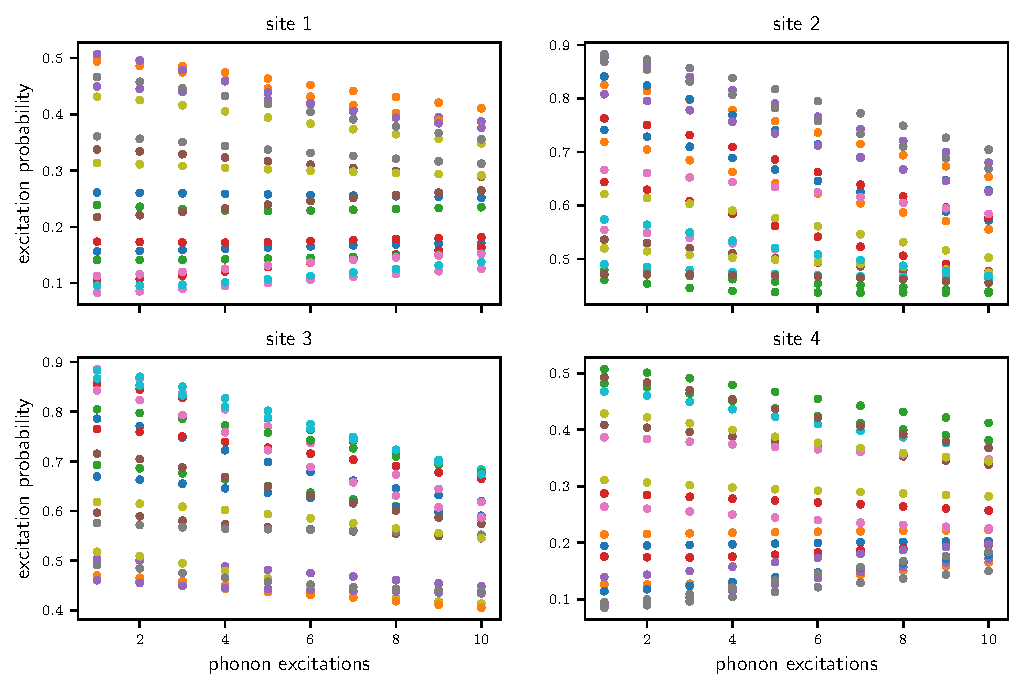
\includegraphics[scale=0.99]{pictures/chain4_maxima_dep_phnumb.pdf}
    % \caption{\textbf{spin-phonon coupling only.}}
    % \label{fig:fidelity}
\end{figure}
\begin{figure}[H]
    \hspace*{-2.5cm}
    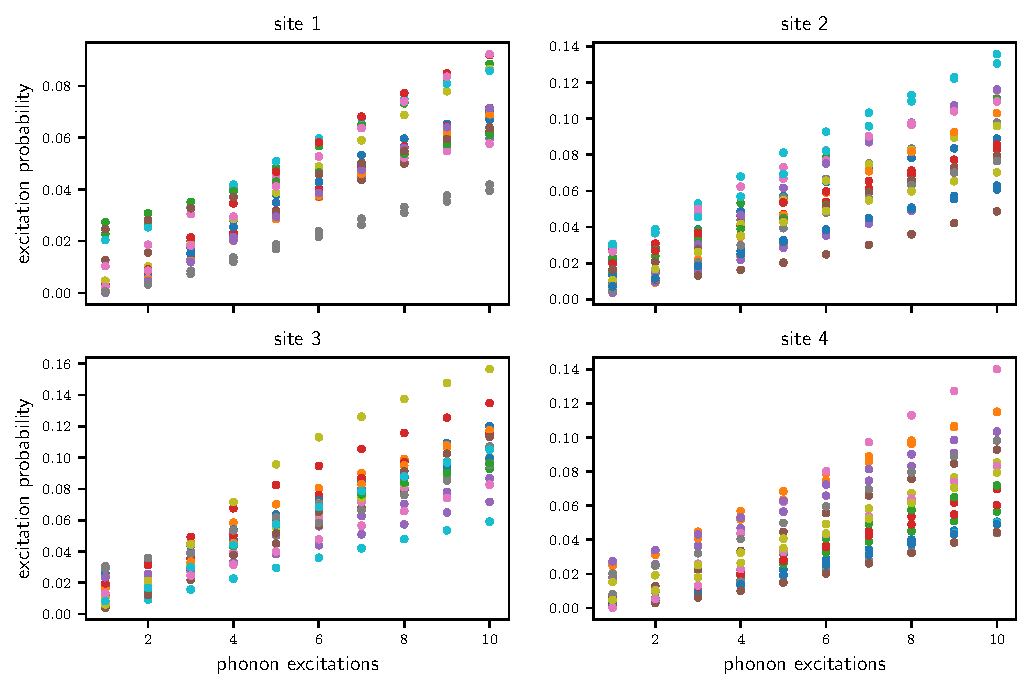
\includegraphics[scale=0.99]{pictures/chain4_minima_dep_phnumb.pdf}
    % \caption{\textbf{spin-phonon coupling only.}}
    % \label{fig:fidelity}
\end{figure}
\begin{figure}[H]
    \hspace*{-2.5cm}
    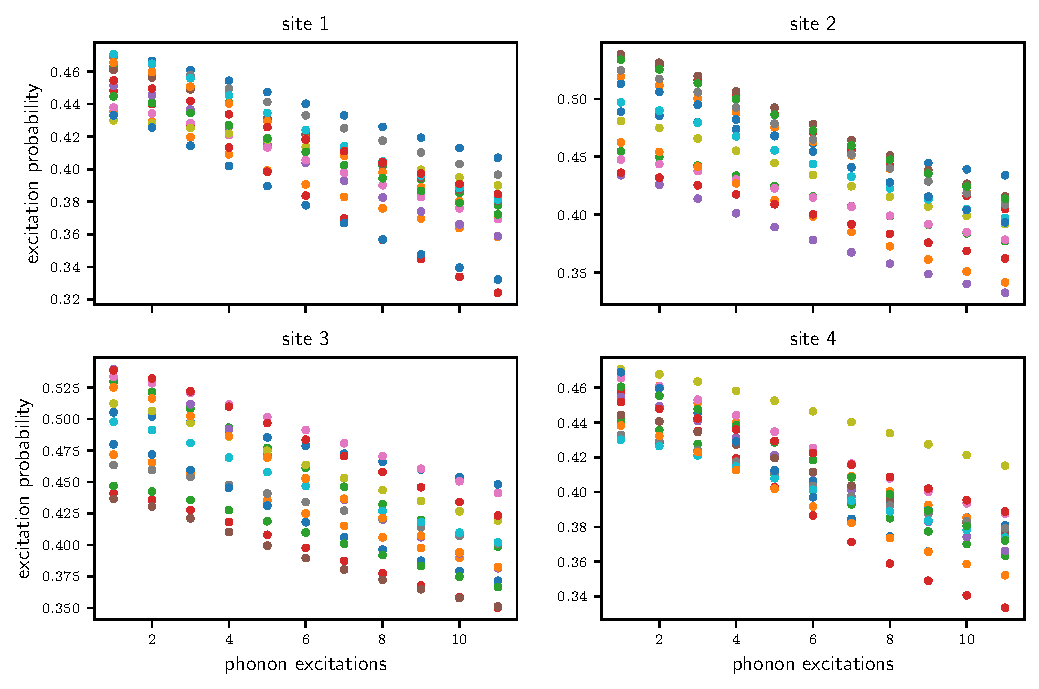
\includegraphics[scale=0.99]{pictures/chain4_maxima_dep_phnumb2.pdf}
    % \caption{\textbf{spin-phonon coupling only.}}
    % \label{fig:fidelity}
\end{figure}
\begin{figure}[H]
    \hspace*{-2.5cm}
    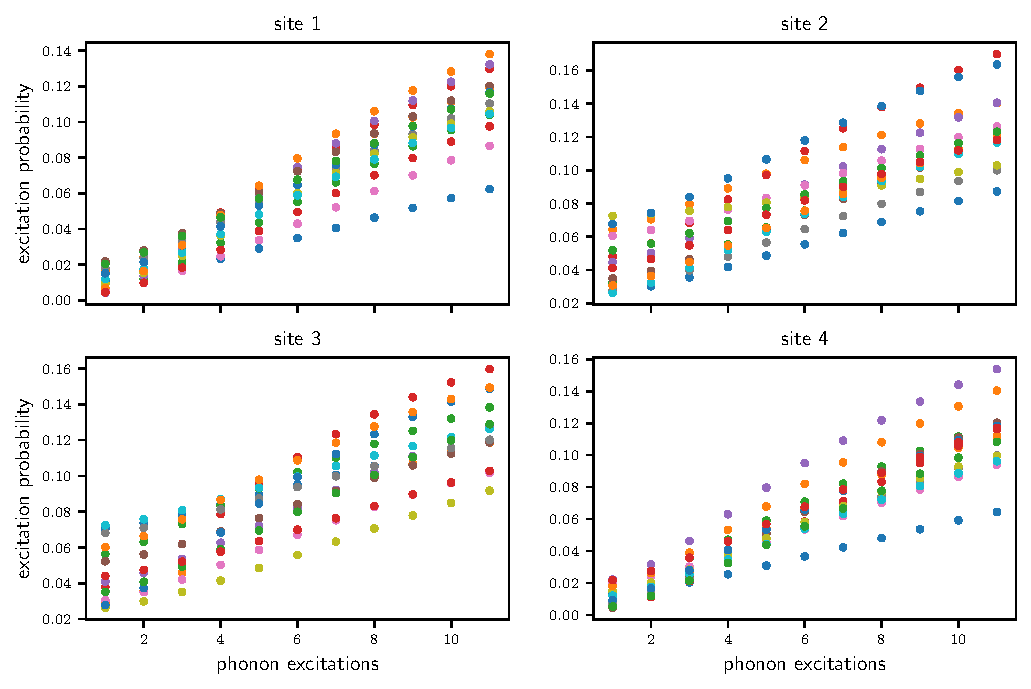
\includegraphics[scale=0.99]{pictures/chain4_minima_dep_phnumb2.pdf}
    % \caption{\textbf{spin-phonon coupling only.}}
    % \label{fig:fidelity}
\end{figure}

\begin{figure}[H]
    \hspace*{-2.5cm}
    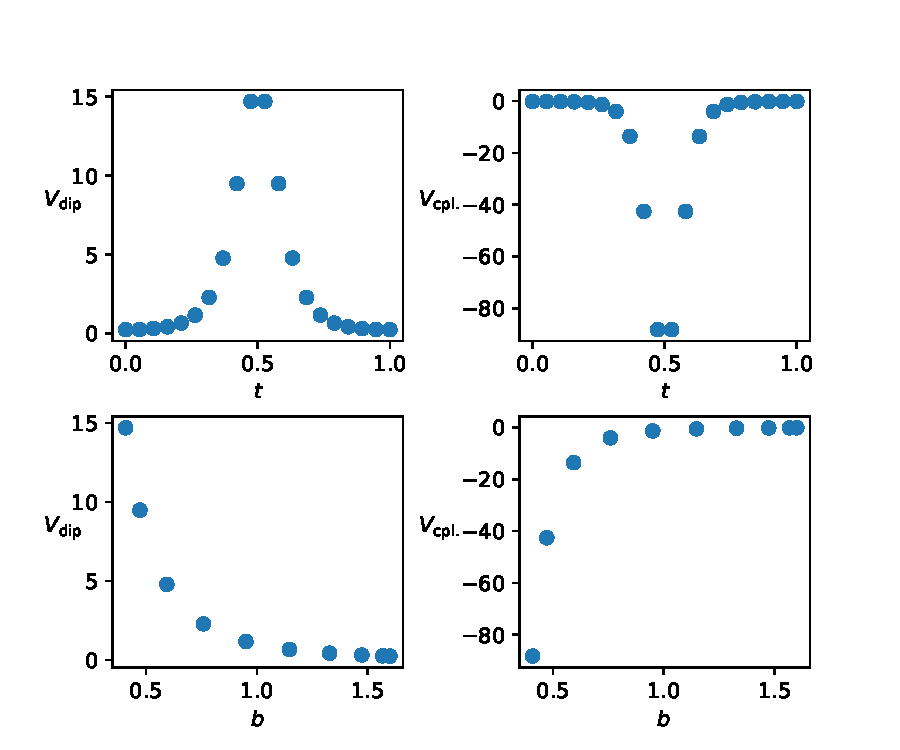
\includegraphics[scale=1]{pictures/interaction_ricemele_chain4.pdf}
    \caption{\textbf{Interaction strengths during Rice-Mele scheme.}}
    % \label{fig:fidelity}
\end{figure}
\begin{figure}[H]
    \hspace*{-2.5cm}
    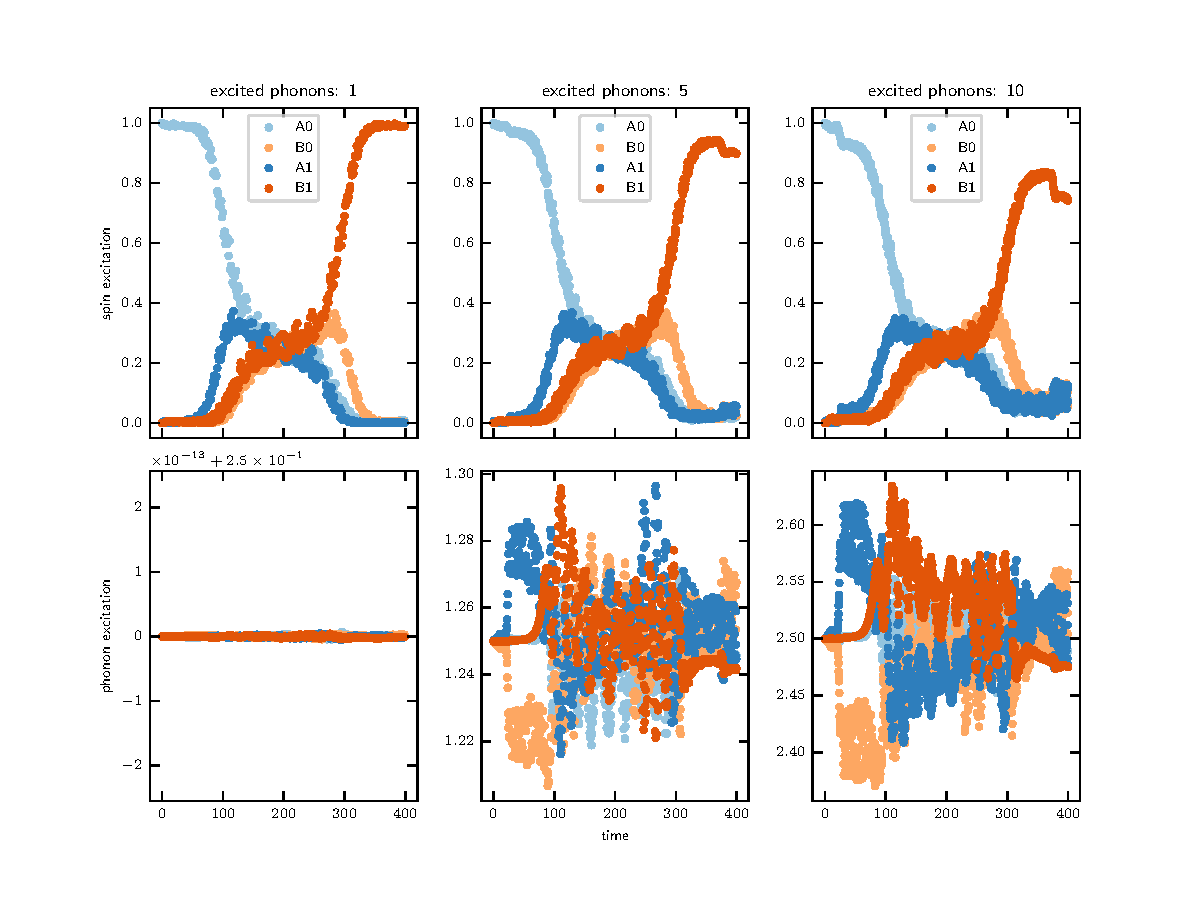
\includegraphics{pictures/chain4_ricemele_1spto10oupling.pdf}
    \caption{\textbf{Rice-Mele scheme.}}
    % \label{fig:fidelity}
\end{figure}
% \begin{figure}[H]
%     \begin{subfig}{0.5\textwidth}
%         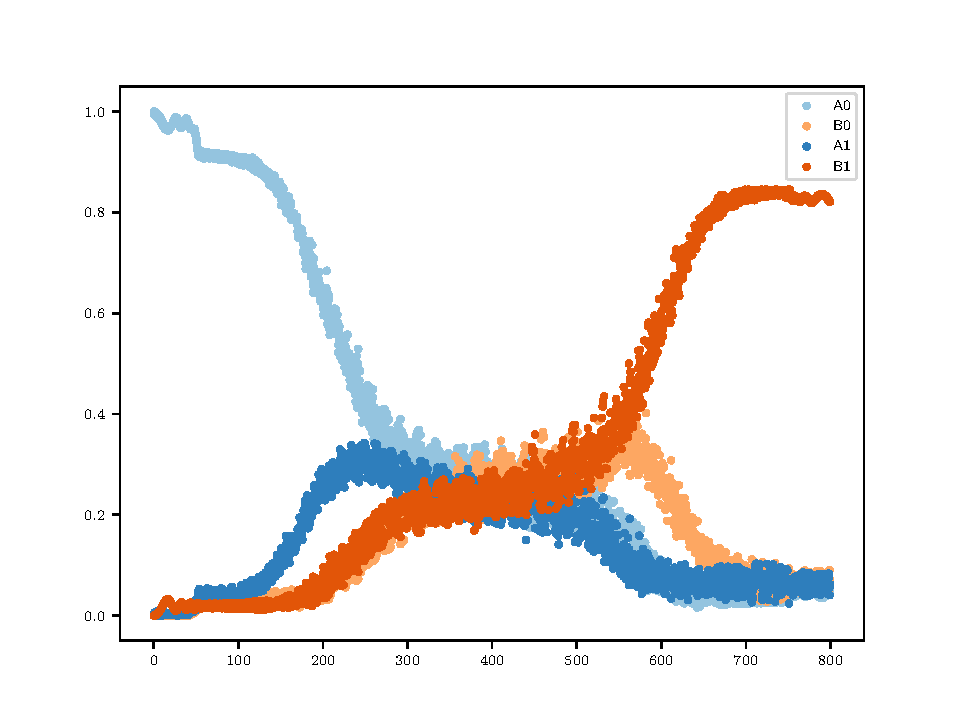
\includegraphics[scale=1]{pictures/chain4_ricemele_1spto10oupling_doubletime_10phonons.pdf.pdf}
%         \caption{\textbf{Rice-Mele scheme with longer time evolution.}}
%     \end{subfig}
%     \begin{subfig}{0.5\textwidth}
%         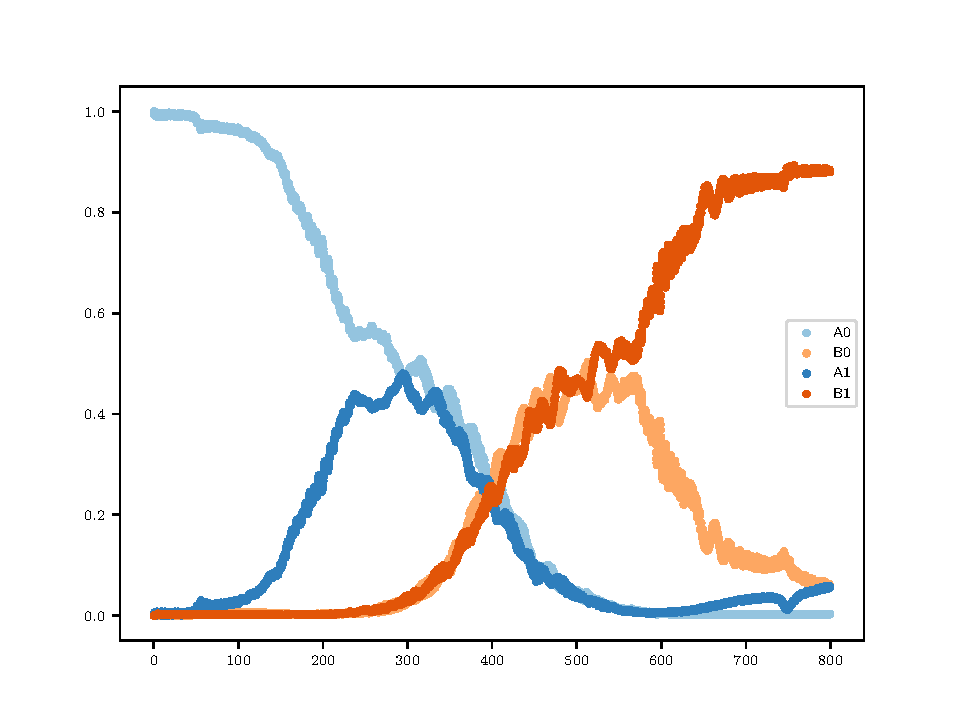
\includegraphics[scale=1]{pictures/chain4_ricemele_1spto10oupling_doubletime_10phonons_Delta10.pdf}
%         \caption{\textbf{Rice-Mele scheme with longer time evolution with $\Delta$ 10 times higher.}}
%     \end{subfig}
% \end{figure}
\begin{figure}[H]
    \centering

    % --- Left subplot ---
    \begin{subfigure}[b]{0.48\textwidth}
        \centering
        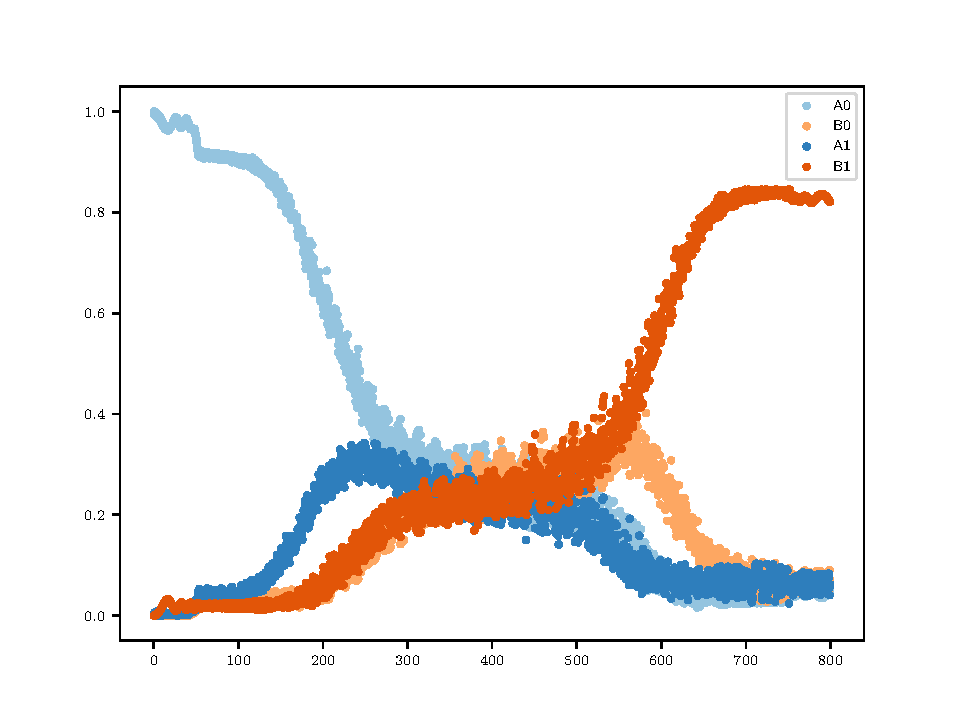
\includegraphics[width=\textwidth]{pictures/chain4_ricemele_1spto10oupling_doubletime_10phonons.pdf}
        \caption{$\Delta=1$}
        \label{fig:image1}
    \end{subfigure}
    \hfill
    % --- Right subplot ---
    \begin{subfigure}[b]{0.48\textwidth}
        \centering
        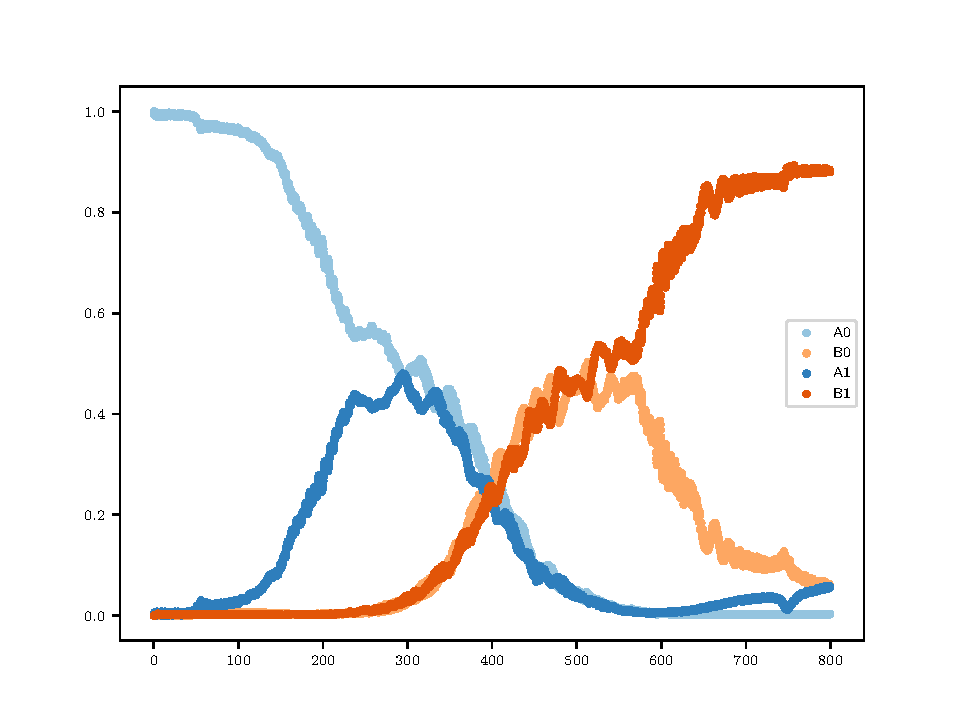
\includegraphics[width=\textwidth]{pictures/chain4_ricemele_1spto10oupling_doubletime_10phonons_Delta10.pdf}
        \caption{$\Delta=10$}
        \label{fig:image2}
    \end{subfigure}

    \caption{\textbf{longer time evolution for phonon number 10.}}
    \label{fig:both}
\end{figure}
